\documentclass[openany]{tufte-book} % Use the tufte-book class which in turn uses the tufte-common class
\hypersetup{colorlinks} % Comment this line if you don't wish to have colored links
\usepackage{microtype} % Improves character and word spacing
\usepackage{booktabs} % Better horizontal rules in tables
\usepackage{tkz-graph}
\usepackage{graphicx} % Needed to insert images into the document
\graphicspath{{graphics/}} % Sets the default location of pictures
\setkeys{Gin}{width=\linewidth,totalheight=\textheight,keepaspectratio} % Improves figure scaling

\usepackage{fancyvrb} % Allows customization of verbatim environments
\fvset{fontsize=\normalsize} % The font size of all verbatim text can be changed here

\newcommand{\hangp}[1]{\makebox[0pt][r]{(}#1\makebox[0pt][l]{)}} % New command to create parentheses around text in tables which take up no horizontal space - this improves column spacing
\newcommand{\hangstar}{\makebox[0pt][l]{*}} % New command to create asterisks in tables which take up no horizontal space - this improves column spacing

\usepackage{xspace} % Used for printing a trailing space better than using a tilde (~) using the \xspace command

\newcommand{\monthyear}{\ifcase\month\or January\or February\or March\or April\or May\or June\or July\or August\or September\or October\or November\or December\fi\space\number\year} % A command to print the current month and year

\newcommand{\openepigraph}[2]{ % This block sets up a command for printing an epigraph with 2 arguments - the quote and the author
\begin{fullwidth}
\sffamily\large
\begin{doublespace}
\noindent\allcaps{#1}\\ % The quote
\noindent\allcaps{#2} % The author
\end{doublespace}
\end{fullwidth}
}

\newcommand{\blankpage}{\newpage\hbox{}\thispagestyle{empty}\newpage} % Command to insert a blank page

\usepackage{units} % Used for printing standard units

\newcommand{\hlred}[1]{\textcolor{Maroon}{#1}} % Print text in maroon
\newcommand{\hangleft}[1]{\makebox[0pt][r]{#1}} % Used for printing commands in the index, moves the slash left so the command name aligns with the rest of the text in the index 
\newcommand{\hairsp}{\hspace{1pt}} % Command to print a very short space
\newcommand{\ie}{\textit{i.\hairsp{}e.}\xspace} % Command to print i.e.
\newcommand{\eg}{\textit{e.\hairsp{}g.}\xspace} % Command to print e.g.
\newcommand{\na}{\quad--} % Used in tables for N/A cells
\newcommand{\measure}[3]{#1/#2$\times$\unit[#3]{pc}} % Typesets the font size, leading, and measure in the form of: 10/12x26 pc.
\newcommand{\tuftebs}{\symbol{'134}} % Command to print a backslash in tt type in OT1/T1

\providecommand{\XeLaTeX}{X\lower.5ex\hbox{\kern-0.15em\reflectbox{E}}\kern-0.1em\LaTeX}
\newcommand{\tXeLaTeX}{\XeLaTeX\index{XeLaTeX@\protect\XeLaTeX}} % Command to print the XeLaTeX logo while simultaneously adding the position to the index

\newcommand{\doccmdnoindex}[2][]{\texttt{\tuftebs#2}} % Command to print a command in texttt with a backslash of tt type without inserting the command into the index

\newcommand{\doccmddef}[2][]{\hlred{\texttt{\tuftebs#2}}\label{cmd:#2}\ifthenelse{\isempty{#1}} % Command to define a command in red and add it to the index
{ % If no package is specified, add the command to the index
\index{#2 command@\protect\hangleft{\texttt{\tuftebs}}\texttt{#2}}% Command name
}
{ % If a package is also specified as a second argument, add the command and package to the index
\index{#2 command@\protect\hangleft{\texttt{\tuftebs}}\texttt{#2} (\texttt{#1} package)}% Command name
\index{#1 package@\texttt{#1} package}\index{packages!#1@\texttt{#1}}% Package name
}}

\newcommand{\doccmd}[2][]{% Command to define a command and add it to the index
\texttt{\tuftebs#2}%
\ifthenelse{\isempty{#1}}% If no package is specified, add the command to the index
{%
\index{#2 command@\protect\hangleft{\texttt{\tuftebs}}\texttt{#2}}% Command name
}
{%
\index{#2 command@\protect\hangleft{\texttt{\tuftebs}}\texttt{#2} (\texttt{#1} package)}% Command name
\index{#1 package@\texttt{#1} package}\index{packages!#1@\texttt{#1}}% Package name
}}

% A bunch of new commands to print commands, arguments, environments, classes, etc within the text using the correct formatting
\newcommand{\docopt}[1]{\ensuremath{\langle}\textrm{\textit{#1}}\ensuremath{\rangle}}
\newcommand{\docarg}[1]{\textrm{\textit{#1}}}
\newenvironment{docspec}{\begin{quotation}\ttfamily\parskip0pt\parindent0pt\ignorespaces}{\end{quotation}}
\newcommand{\docenv}[1]{\texttt{#1}\index{#1 environment@\texttt{#1} environment}\index{environments!#1@\texttt{#1}}}
\newcommand{\docenvdef}[1]{\hlred{\texttt{#1}}\label{env:#1}\index{#1 environment@\texttt{#1} environment}\index{environments!#1@\texttt{#1}}}
\newcommand{\docpkg}[1]{\texttt{#1}\index{#1 package@\texttt{#1} package}\index{packages!#1@\texttt{#1}}}
\newcommand{\doccls}[1]{\texttt{#1}}
\newcommand{\docclsopt}[1]{\texttt{#1}\index{#1 class option@\texttt{#1} class option}\index{class options!#1@\texttt{#1}}}
\newcommand{\docclsoptdef}[1]{\hlred{\texttt{#1}}\label{clsopt:#1}\index{#1 class option@\texttt{#1} class option}\index{class options!#1@\texttt{#1}}}
\newcommand{\docmsg}[2]{\bigskip\begin{fullwidth}\noindent\ttfamily#1\end{fullwidth}\medskip\par\noindent#2}
\newcommand{\docfilehook}[2]{\texttt{#1}\index{file hooks!#2}\index{#1@\texttt{#1}}}
\newcommand{\doccounter}[1]{\texttt{#1}\index{#1 counter@\texttt{#1} counter}}

\usepackage{remreset}% to allow continuous numbering of figures/tables throughout the entire book

\makeatletter% since we're using commands with @ in their name
\@removefromreset{figure}{chapter}% don't reset figure numbering
\@removefromreset{table}{chapter}% don't reset figure numbering
\let\origappendix\appendix% save a copy of the original meaning of \appendix
\renewcommand{\appendix}{%
  \origappendix% do all the original \appendix stuff
  \titlecontents{chapter}%
    [0em] % distance from left margin
    {\vspace{1.5\baselineskip}\begin{fullwidth}\LARGE\rmfamily\itshape} % above (global formatting of entry)
    {\hspace*{0em}\appendixname~\thecontentslabel: } % before w/label (label = ``2'')
    {\hspace*{0em}} % before w/o label
    {\rmfamily\upshape\qquad\thecontentspage} % filler + page (leaders and page num)
    [\end{fullwidth}] % after
  \titleformat{\chapter}%
    [display]% shape
    {\relax\ifthenelse{\NOT\boolean{@tufte@symmetric}}{\begin{fullwidth}}{}}% format applied to label+text
    {\itshape\huge Appendix~\thechapter}% label
    {0pt}% horizontal separation between label and title body
    {\huge\rmfamily\itshape}% before the title body
    [\ifthenelse{\NOT\boolean{@tufte@symmetric}}{\end{fullwidth}}{}]% after the title body
  \setcounter{secnumdepth}{0}% ``number'' the appendices
  \renewcommand{\thefigure}{\@arabic\c@figure}% define \thefigure to use only the figure number (1), not A.1
  \renewcommand{\thetable}{\@arabic\c@table}%
  %
  % Add any other special appendix-related code here.
  %
}
\makeatother% restore the special meaning of @

\usepackage{makeidx} % Used to generate the index
\makeindex % Generate the index which is printed at the end of the document


\usepackage{amsmath, amsthm, amssymb}
\theoremstyle{plain}
\newtheorem{acknowledgement}{Acknowledgement}
\newtheorem{algorithm}{Algorithm}
\newtheorem{axiom}{Axiom}
\newtheorem{case}{Case}
\newtheorem{claim}{Claim}
\newtheorem{conclusion}{Conclusion}
\newtheorem{condition}{Condition}
\newtheorem{conjecture}{Conjecture}
\newtheorem{corollary}{Corollary}
\newtheorem{criterion}{Criterion}
\newtheorem{definition}{Definition}
\newtheorem{example}{Example}
\newtheorem{exercise}{Exercise}
\newtheorem{lemma}{Lemma}
\newtheorem{notation}{Notation}
\newtheorem{problem}{Problem}
\newtheorem{proposition}{Proposition}
\newtheorem{remark}{Remark}
\newtheorem{observation}{Observation}
\newtheorem{question}{Question}
\newtheorem{solution}{Solution}
\newtheorem{summary}{Summary}
\newtheorem{theorem}{Theorem}

\newcommand{\set}[1]{\left\{ #1 \right\}}
\newcommand{\setb}[3]{\left\{ #1 \in #2 : #3 \right\}}
\newcommand{\setbs}[2]{\left\{ #1 : #2 \right\}}
\newcommand{\card}[1]{\left|#1\right|}
\newcommand{\size}[1]{\left\Vert#1\right\Vert}
\newcommand{\ceil}[1]{\left\lceil#1\right\rceil}
\newcommand{\floor}[1]{\left\lfloor#1\right\rfloor}
\newcommand{\func}[3]{#1\colon #2 \rightarrow #3}
\newcommand{\funcinj}[3]{#1\colon #2 \inj #3}
\newcommand{\funcsurj}[3]{#1\colon #2 \surj #3}
\newcommand{\irange}[1]{\left[#1\right]}
\newcommand{\join}[2]{#1 \mbox{\hspace{2 pt}$\ast$\hspace{2 pt}} #2}
\newcommand{\djunion}[2]{#1 \mbox{\hspace{2 pt}$+$\hspace{2 pt}} #2}
\newcommand{\parens}[1]{\left( #1 \right)}
\newcommand{\brackets}[1]{\left[ #1 \right]}
\newcommand{\DefinedAs}{\mathrel{\mathop:}=}

\newcommand{\Q}{\mathbb{Q}}
\newcommand{\fancy}[1]{\mathcal{#1}}
\newcommand{\C}[1]{\fancy{C}_{#1}}
\newcommand{\IN}{\mathbb{N}}
\newcommand{\IR}{\mathbb{R}}
\newcommand{\G}{\fancy{G}}
\newcommand{\CC}{\fancy{C}}
\newcommand{\D}{\fancy{D}}
\newcommand{\T}{\fancy{T}}
\newcommand{\B}{\fancy{B}}
\renewcommand{\L}{\fancy{L}}
\newcommand{\HH}{\fancy{H}}

\newcommand{\pot}{\operatorname{pot}}

\usepackage{makeidx} % Used to generate the index
\makeindex % Generate the index which is printed at the end of the document
\title{Basic Graph Coloring}
\author{landon rabern}

\begin{document}

\frontmatter
\maketitle 


\tableofcontents


\cleardoublepage
~\vfill
\begin{doublespace}
\noindent\fontsize{18}{22}\selectfont\itshape
\nohyphenation
For Rachel, Atticus and Alfred.
\end{doublespace}
\vfill
\vfill

\cleardoublepage
\mainmatter
\chapter{Graphs}
A \emph{graph} is a collection of dots we call \emph{vertices} some of which are connected by curves we call \emph{edges}. 
The relative location of the dots and the shape of the curves are not relevant, we are only concerned with whether or not a given
pair of dots is connected by a curve.  Initially, we forbid edges from a vertex to itself and multiple edges between two vertices.
If $G$ is a graph, then $V(G)$ is its set of vertices and $E(G)$ its set of edges. 
We write $\card{G}$ for the number of vertices in $V(G)$ and $\size{G}$ for the number of edges in $E(G)$.
Two vertices
are \emph{adjacent}  if they are connected by an edge.  The set
of vertices to which $v$ is adjacent is its \emph{neighborhood}, written $N(v)$. 
For the size of $v$'s neighborhood $\card{N(v)}$, we write $d(v)$ and call this the \emph{degree} of $v$.

We use the shorthand $\irange{k} \DefinedAs \set{1,2,\ldots, k}$. A \emph{path} in $G$ is a sequence of different vertices $x_1, x_2, \ldots, x_r$ such that $x_i$ is adjacent to $x_{i+1}$ for all $i \in \irange{r-1}$.  We say
this is a path from $x_1$ to $x_r$.
If $x_r$ is adjacent to $x_1$ as well, then we have a \emph{cycle}.  A graph $G$ is \emph{connected} if for all $x,y \in V(G)$, there is a path from $x$ to $y$.
Figure \ref{fig:SmallGraphs} shows all the connected graphs with at most five vertices.

\begin{marginfigure}
		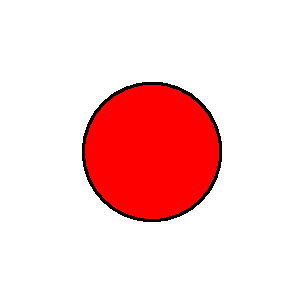
\includegraphics[width=0.5in]{graphs/all/0.pdf}
		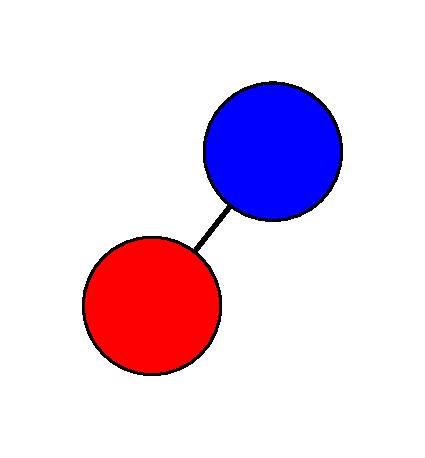
\includegraphics[width=0.5in]{graphs/all/1.pdf}
		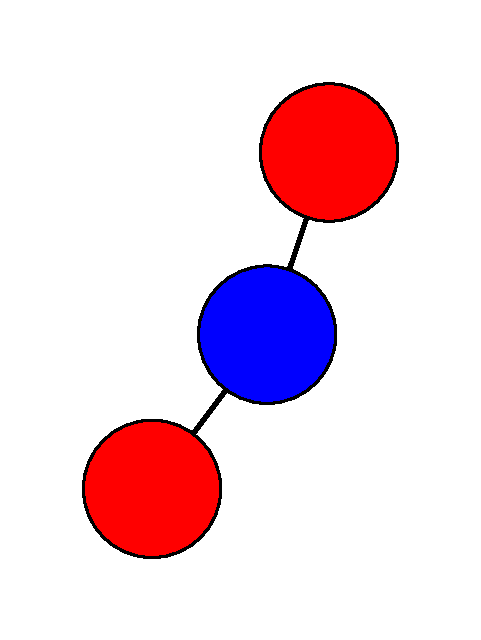
\includegraphics[width=0.5in]{graphs/all/011.pdf}
		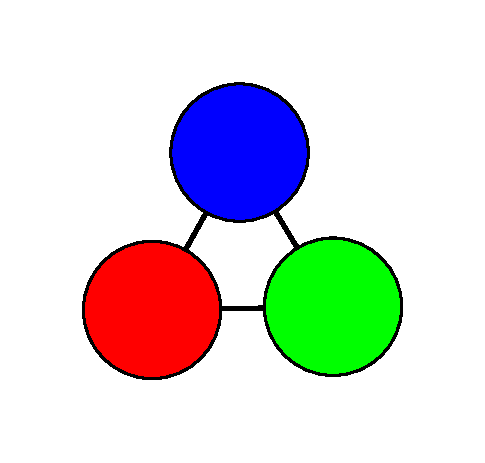
\includegraphics[width=0.5in]{graphs/all/111.pdf}
		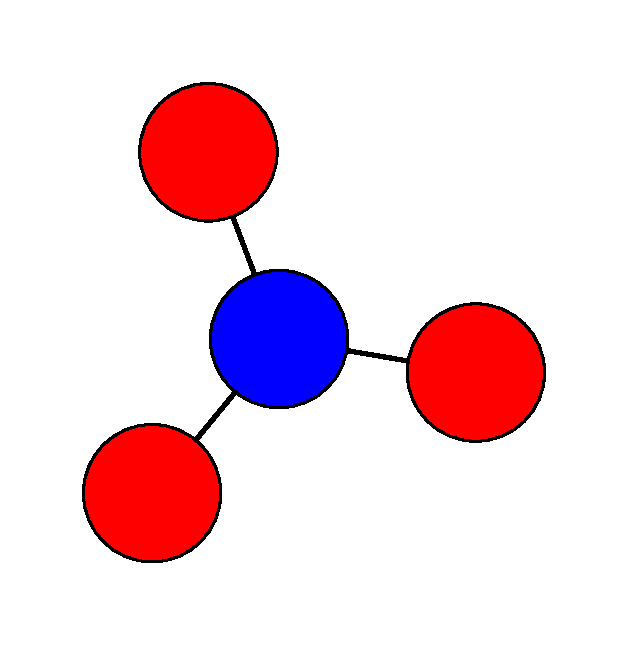
\includegraphics[width=0.5in]{graphs/all/001011.pdf}
		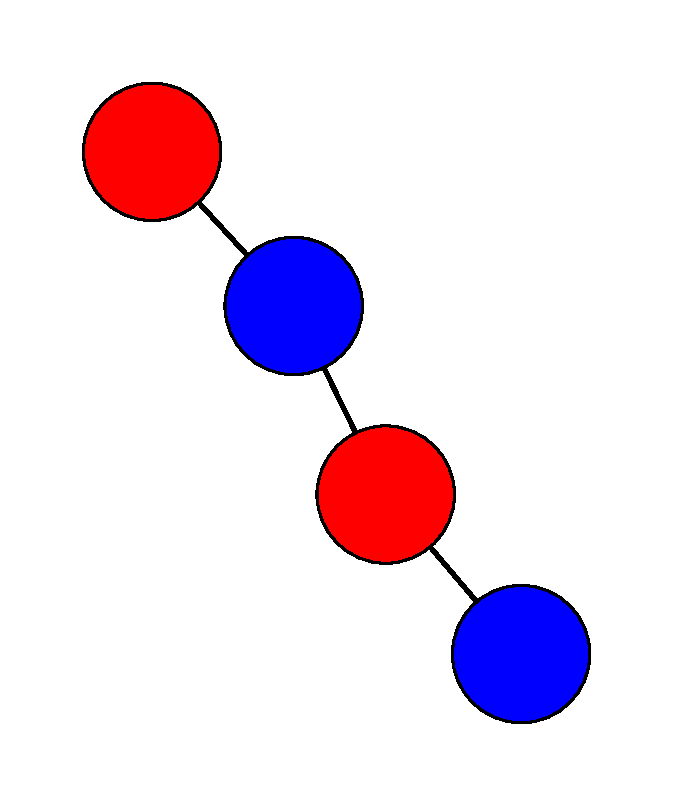
\includegraphics[width=0.5in]{graphs/all/011010.pdf}
		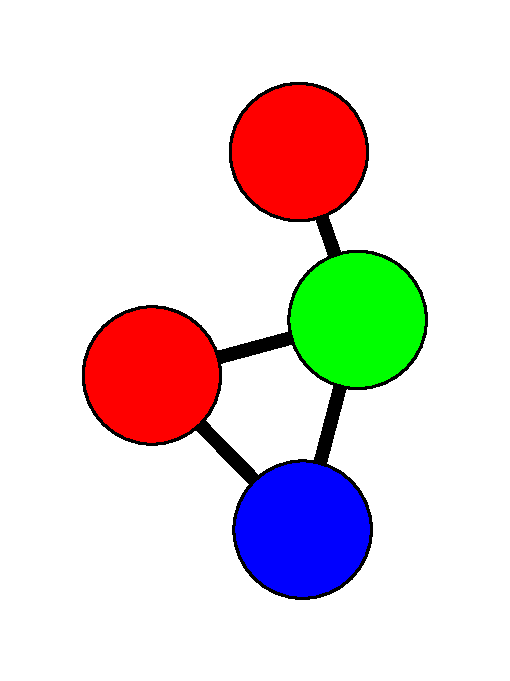
\includegraphics[width=0.5in]{graphs/all/011011.pdf}
		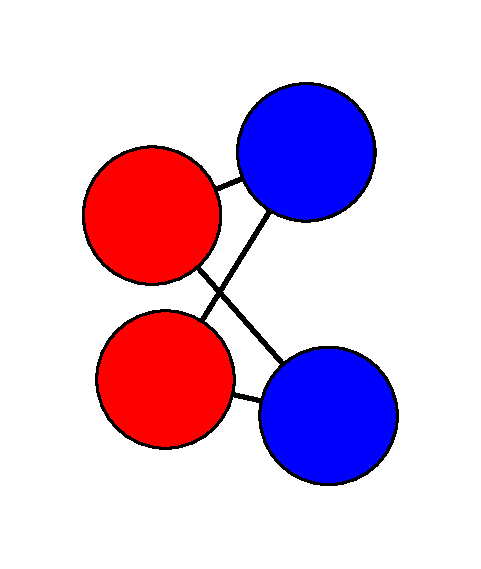
\includegraphics[width=0.5in]{graphs/all/011110.pdf}
		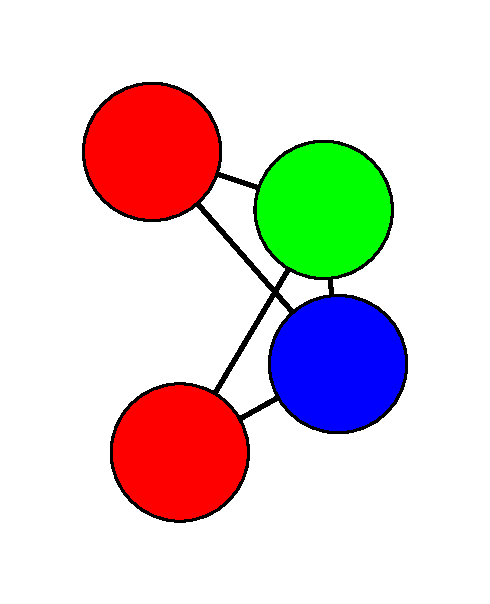
\includegraphics[width=0.5in]{graphs/all/011111.pdf}
		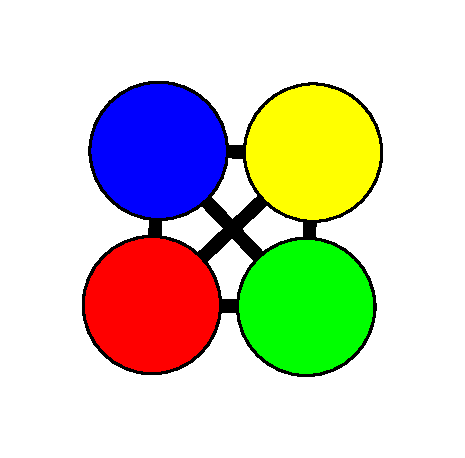
\includegraphics[width=0.5in]{graphs/all/111111.pdf}
		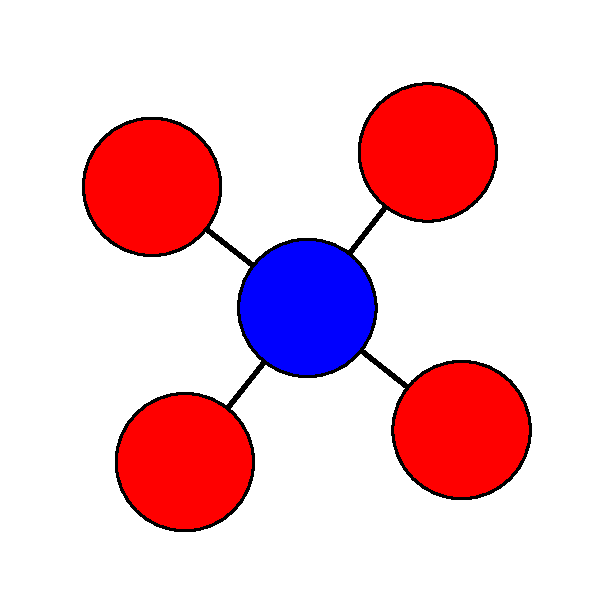
\includegraphics[width=0.5in]{graphs/all/0001001011.pdf}
		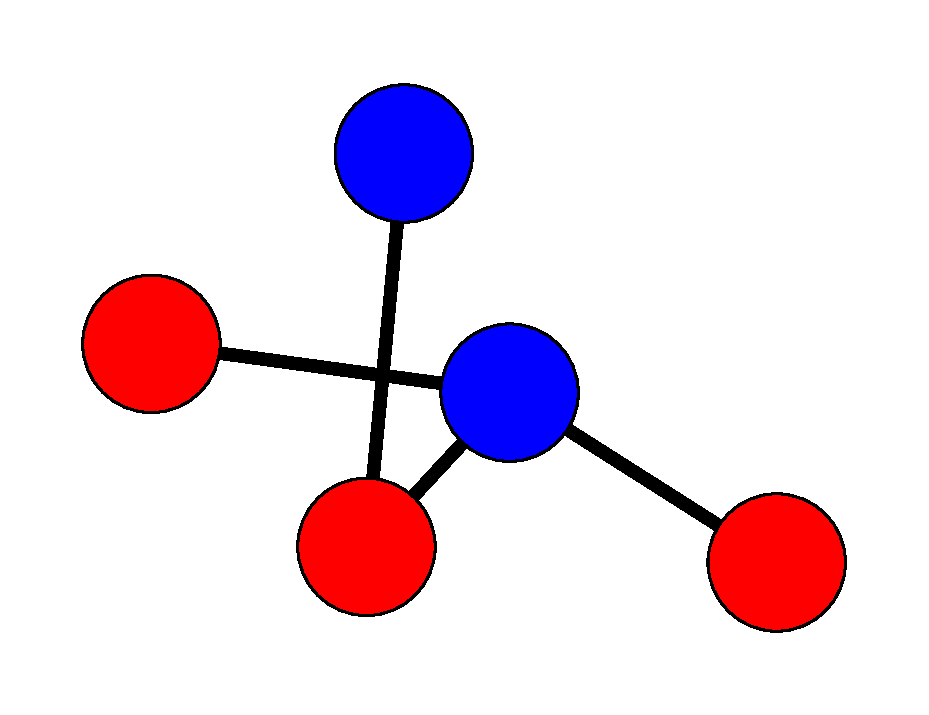
\includegraphics[width=0.5in]{graphs/all/0011001010.pdf}
		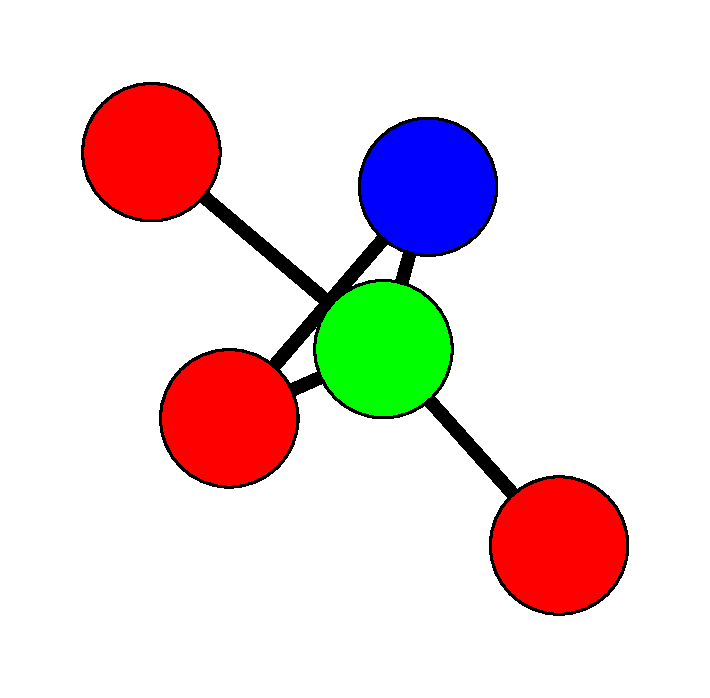
\includegraphics[width=0.5in]{graphs/all/0011001011.pdf}
		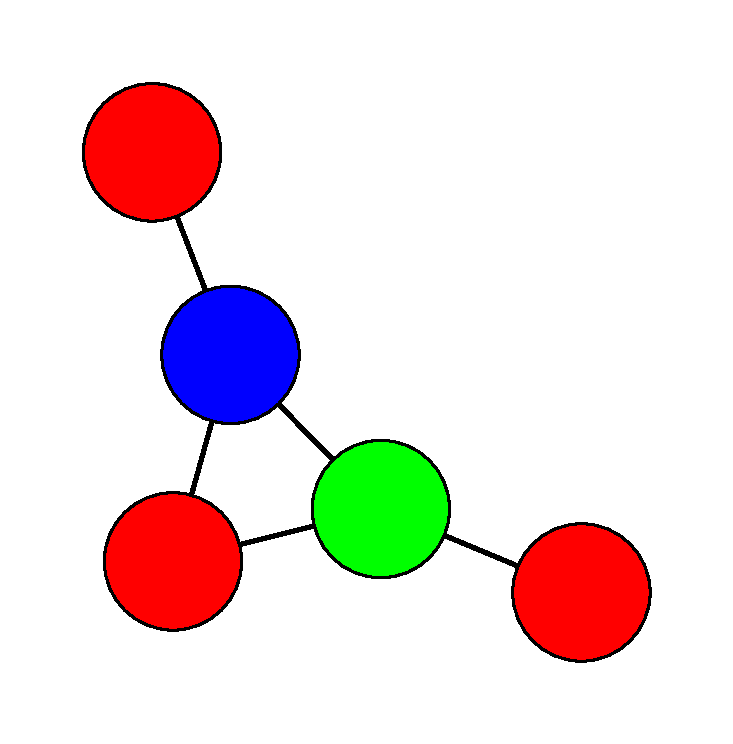
\includegraphics[width=0.5in]{graphs/all/0011010011.pdf}
		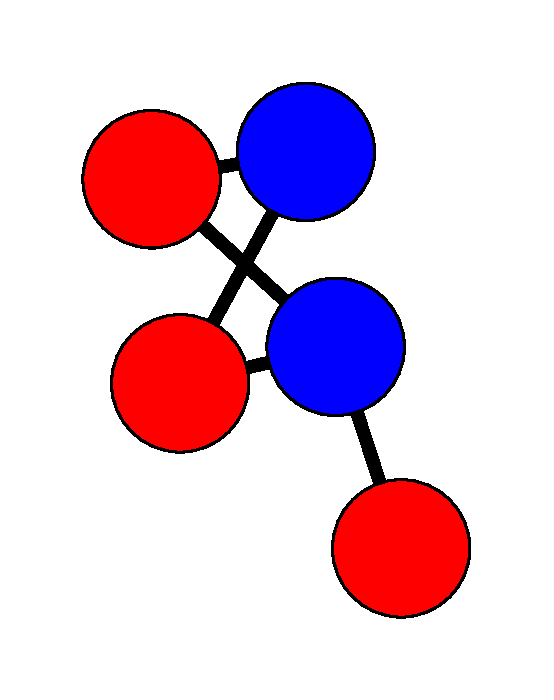
\includegraphics[width=0.5in]{graphs/all/0011011010.pdf}
		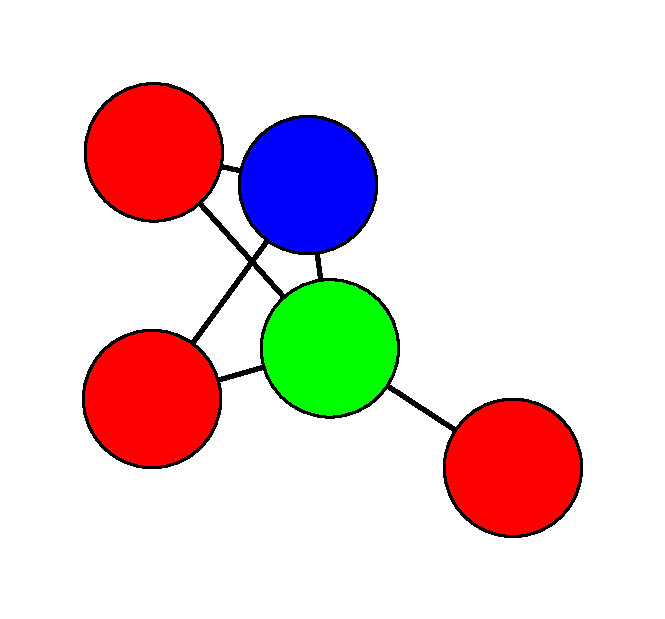
\includegraphics[width=0.5in]{graphs/all/0011011011.pdf}
		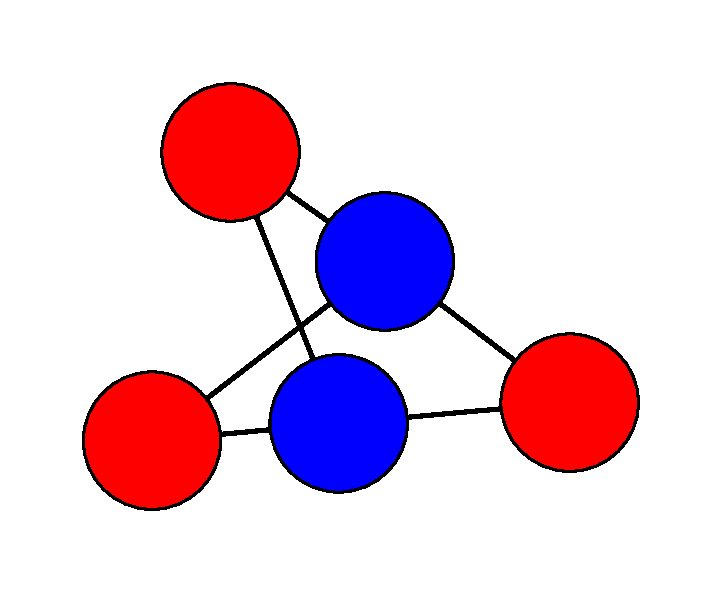
\includegraphics[width=0.5in]{graphs/all/0011011110.pdf}
		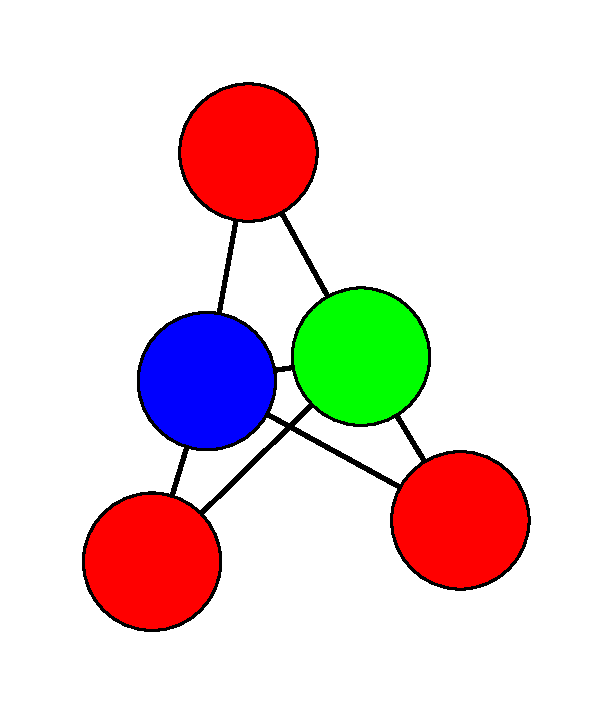
\includegraphics[width=0.5in]{graphs/all/0011011111.pdf}
		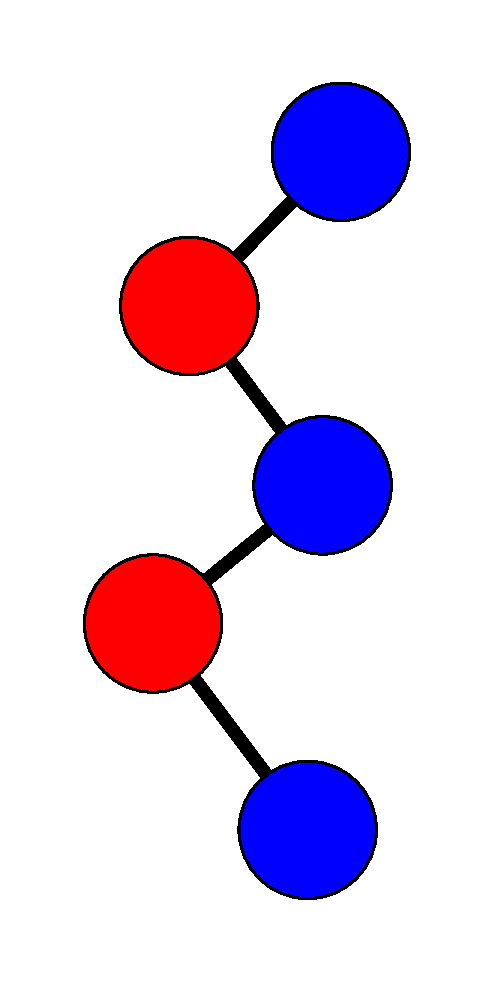
\includegraphics[width=0.5in]{graphs/all/0101011000.pdf}
		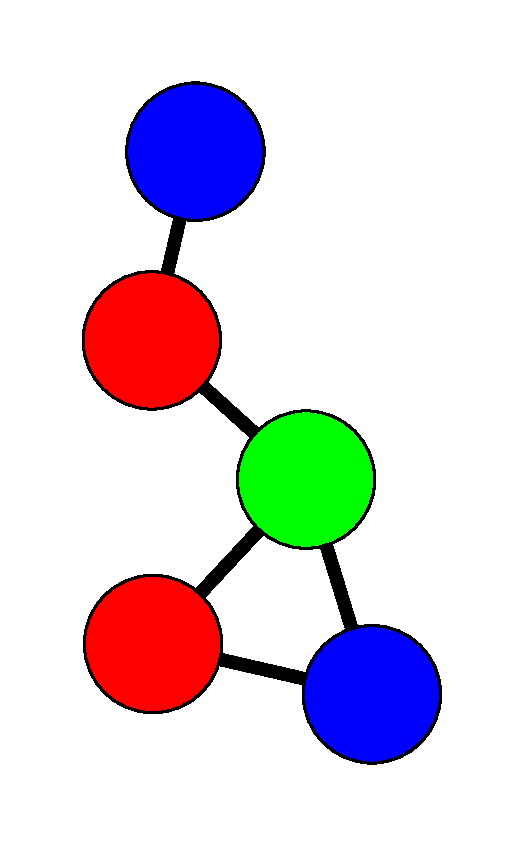
\includegraphics[width=0.5in]{graphs/all/0101011010.pdf}
		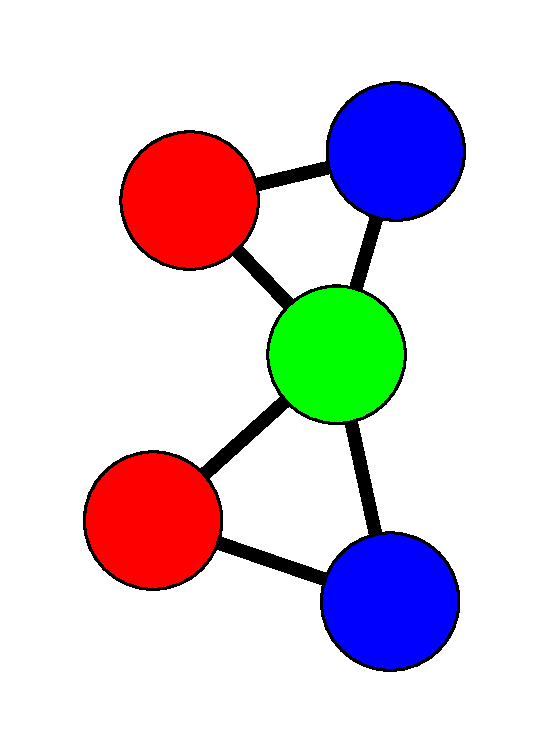
\includegraphics[width=0.5in]{graphs/all/0101011011.pdf}
		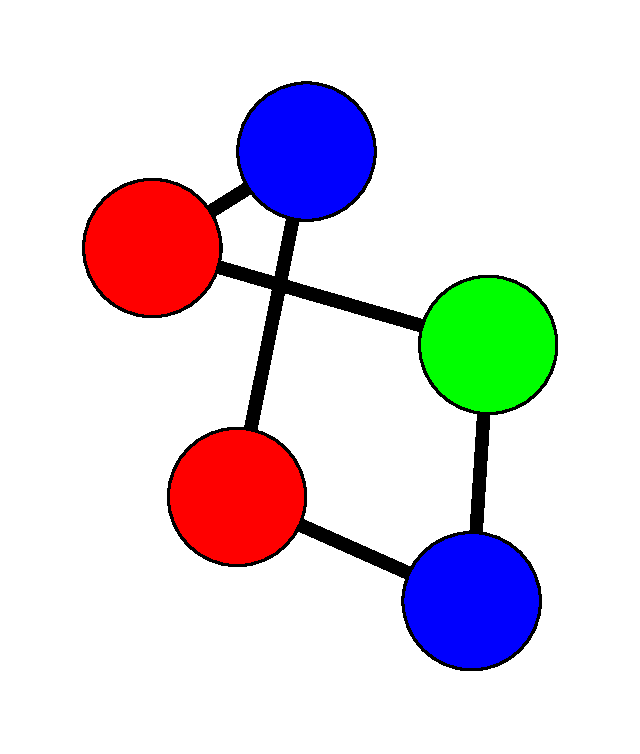
\includegraphics[width=0.5in]{graphs/all/0110011010.pdf}
		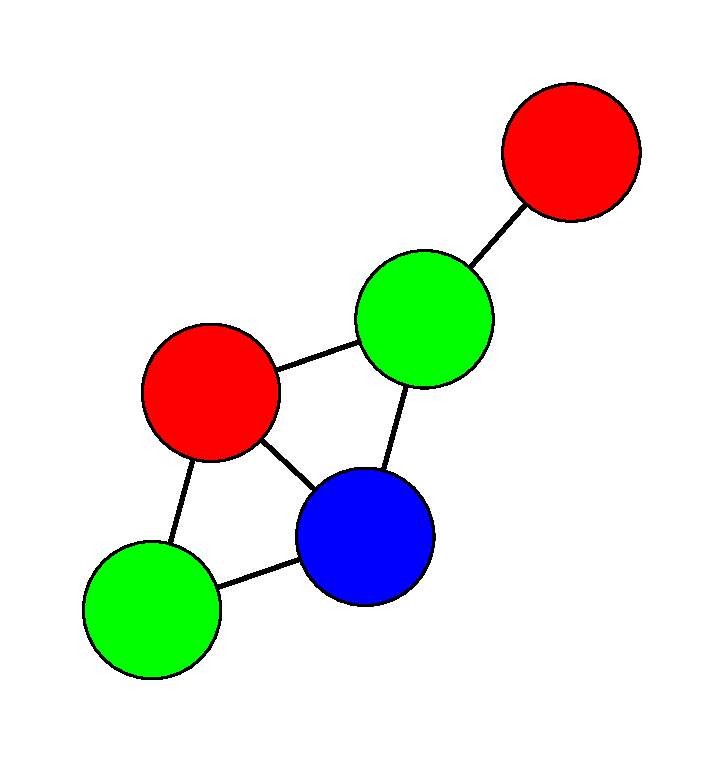
\includegraphics[width=0.5in]{graphs/all/0111001110.pdf}
		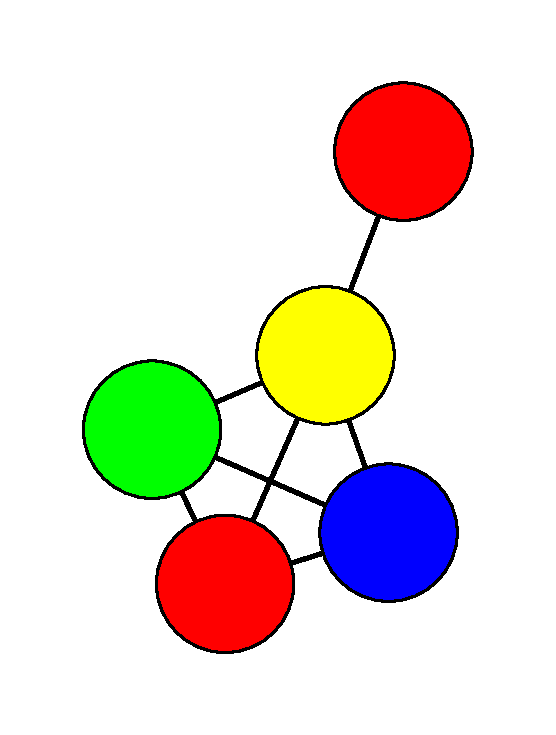
\includegraphics[width=0.5in]{graphs/all/0111001111.pdf}
		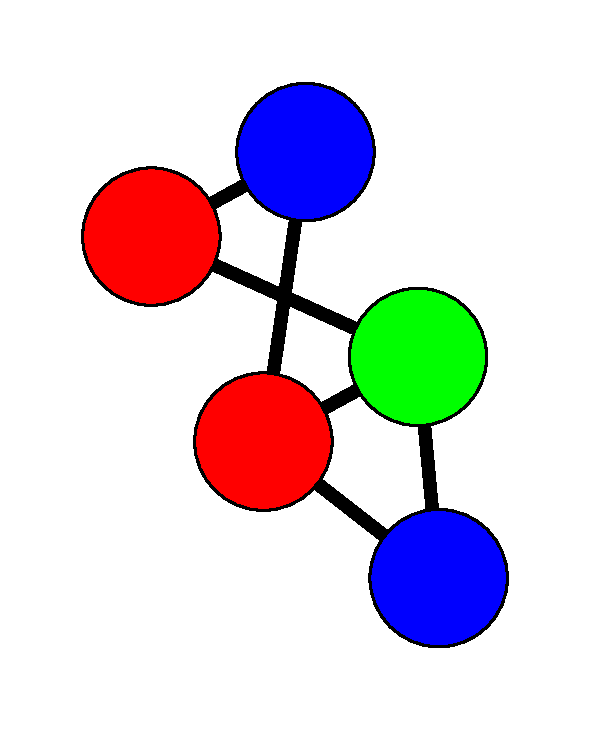
\includegraphics[width=0.5in]{graphs/all/0111011010.pdf}
		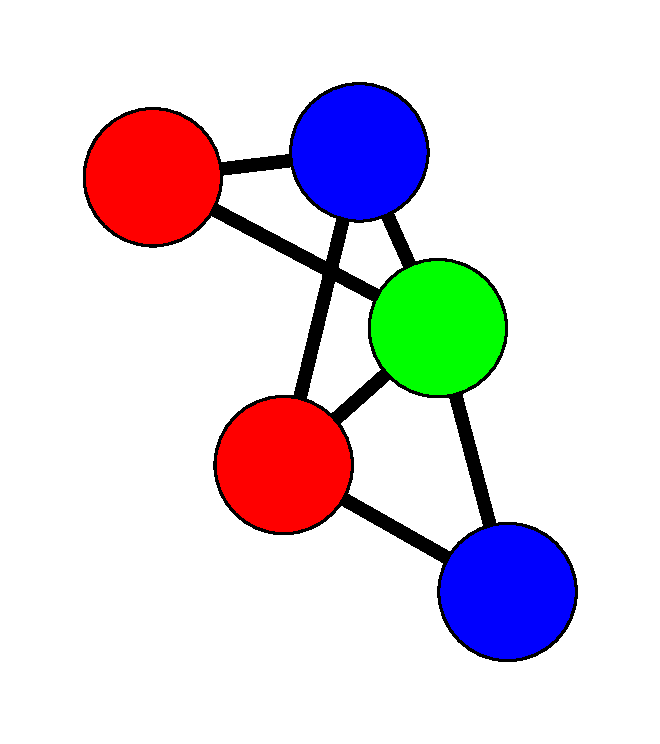
\includegraphics[width=0.5in]{graphs/all/0111011011.pdf}
		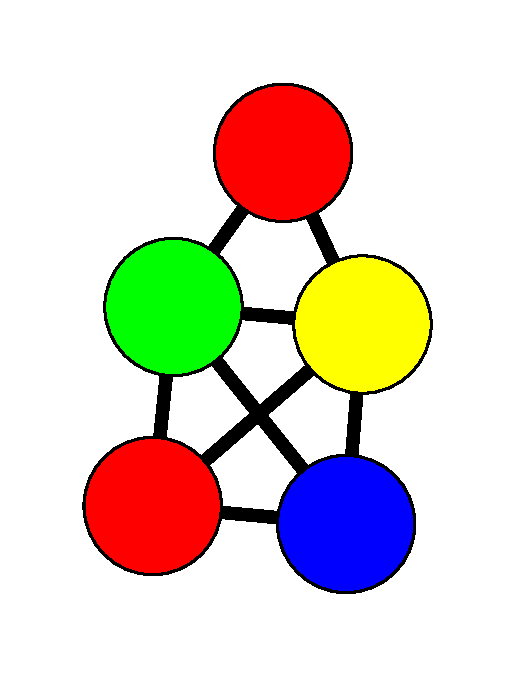
\includegraphics[width=0.5in]{graphs/all/0111011111.pdf}
		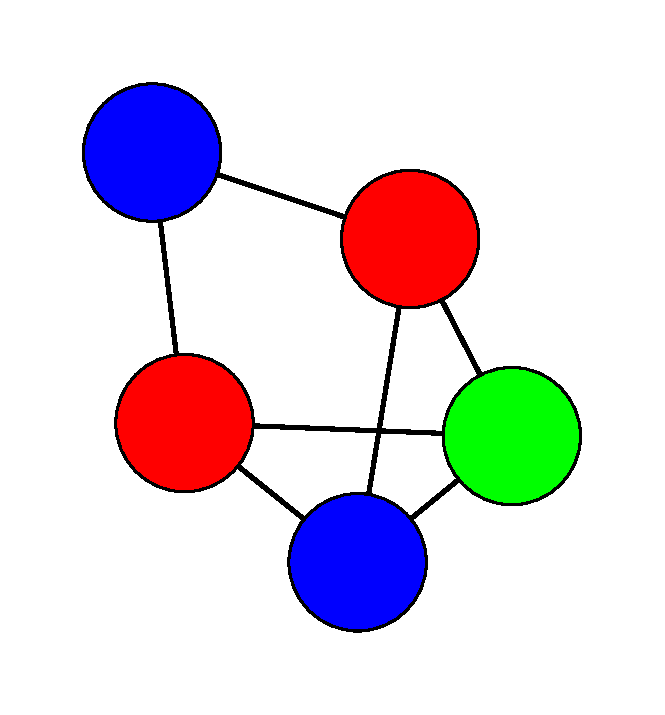
\includegraphics[width=0.5in]{graphs/all/0111111010.pdf}
		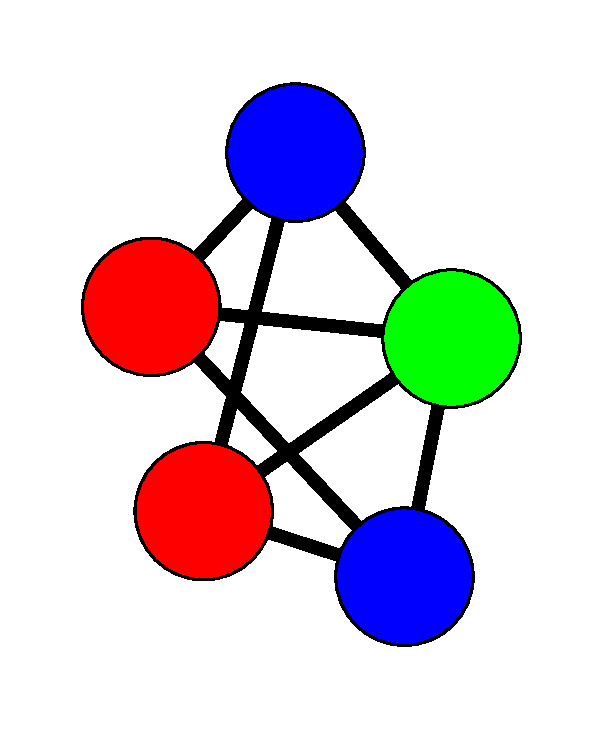
\includegraphics[width=0.5in]{graphs/all/0111111011.pdf}
		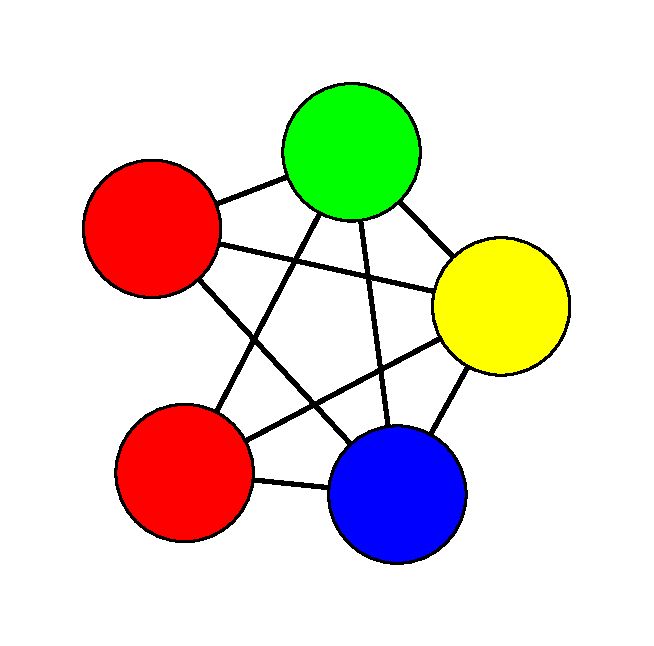
\includegraphics[width=0.5in]{graphs/all/0111111111.pdf}
		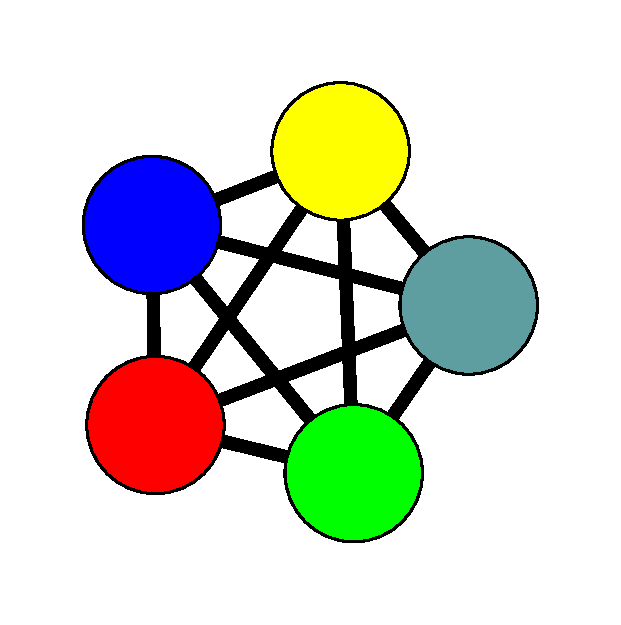
\includegraphics[width=0.5in]{graphs/all/1111111111.pdf}
		\caption{The connected graphs with at most five vertices.}
		\label{fig:SmallGraphs}
\end{marginfigure}

\chapter{Coloring vertices}
\begin{marginfigure}
		
\includegraphics[width=2.5in]{pictures/crayons.png}
		\caption{These are crayons.}
\end{marginfigure}

The entire book concerns one simple task: we want to color the vertices of a given graph so that adjacent vertices receive different colors.
With sufficiently many crayons and no preferences about what the coloring should look like, this is easy, we just use a different crayon for each vertex.  
Things get interesting when we ask how few different crayons we can use.  We are definitely going to need an empty box of crayons and that will only do for the
graph with no vertices at all.  
Given one crayon, we can handle all graphs with no edges.  With two crayons, we can do
any path and any cycle with an even number of vertices.  But, we can't handle a triangle or any other cycle with an odd number of vertices.
\begin{marginfigure}
\caption{A graph with no vertices needs no crayons at all.}
\end{marginfigure}
\begin{marginfigure}[0.25in]
\centering
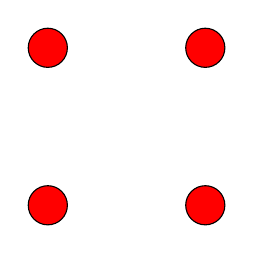
\begin{tikzpicture}[scale = 10]
\tikzstyle{VertexStyle} = []
\tikzstyle{EdgeStyle} = []
\tikzstyle{labeledStyle}=[shape = circle, minimum size = 6pt, inner sep = 1.2pt, draw]
\tikzstyle{unlabeledStyle}=[shape = circle, minimum size = 6pt, inner sep = 1.2pt, draw, fill]
\tikzstyle{c641e27b-ed53-43a3-8b86-e014203f8ed0}=[shape = circle,minimum size = 6pt,inner sep = 5pt,draw,fill={rgb,255:red,255; green,0; blue,0}]
\Vertex[style = c641e27b-ed53-43a3-8b86-e014203f8ed0, x = 0.650, y = 0.700, L = \tiny {}]{v0}
\Vertex[style = c641e27b-ed53-43a3-8b86-e014203f8ed0, x = 0.850, y = 0.700, L = \tiny {}]{v1}
\Vertex[style = c641e27b-ed53-43a3-8b86-e014203f8ed0, x = 0.650, y = 0.500, L = \tiny {}]{v2}
\Vertex[style = c641e27b-ed53-43a3-8b86-e014203f8ed0, x = 0.850, y = 0.500, L = \tiny {}]{v3}
\end{tikzpicture}
\caption{An edgeless graphs needs only one crayon.}
\end{marginfigure}
In fact, odd cycles are really the only thing that will prevent us from using just two crayons. 
A graph $H$ is a \emph{subgraph} of a graph $G$, written $H \subseteq G$ if $V(H) \subseteq V(G)$ and $E(H) \subseteq E(G)$.
When $H \subseteq G$, we say that $G$ \emph{contains} $H$. If $v \in V(G)$, then $G-v$ is the graph we get by removing $v$ and all edges incident to $v$ from $G$.
A graph is $k$-colorable if we can color its vertices with (at most) $k$ colors such that adjacent vertices receive different colors.
A $0$-colorable graph is \emph{empty}, a $1$-colorable graph is \emph{edgeless} and a $2$-colorable graph is \emph{bipartite}.
\begin{marginfigure}[0.25in]
\centering
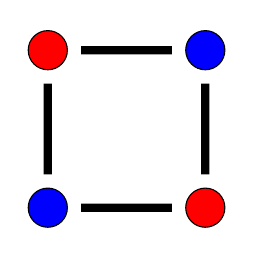
\begin{tikzpicture}[scale = 10]
\tikzstyle{VertexStyle} = []
\tikzstyle{EdgeStyle} = [line width = 3pt]
\tikzstyle{labeledStyle}=[shape = circle, minimum size = 6pt, inner sep = 1.2pt, draw]
\tikzstyle{unlabeledStyle}=[shape = circle, minimum size = 6pt, inner sep = 1.2pt, draw, fill]
\tikzstyle{1b4903bd-d8d6-4bb7-bbf3-64e256860f93}=[shape = circle,minimum size = 6pt,inner sep = 5pt, outer sep = 5pt, draw,fill={rgb,255:red,255; green,0; blue,0}]
\tikzstyle{ab7396a8-c702-4376-a383-e919a68bfd2c}=[shape = circle,minimum size = 6pt,inner sep = 5pt, outer sep = 5pt,draw,fill={rgb,255:red,0; green,0; blue,255}]
\Vertex[style = 1b4903bd-d8d6-4bb7-bbf3-64e256860f93, x = 0.650, y = 0.700, L = \tiny {}]{v0}
\Vertex[style = ab7396a8-c702-4376-a383-e919a68bfd2c, x = 0.850, y = 0.700, L = \tiny {}]{v1}
\Vertex[style = ab7396a8-c702-4376-a383-e919a68bfd2c, x = 0.650, y = 0.500, L = \tiny {}]{v2}
\Vertex[style = 1b4903bd-d8d6-4bb7-bbf3-64e256860f93, x = 0.850, y = 0.500, L = \tiny {}]{v3}
\Edge[label = \tiny {}, labelstyle={auto=right, fill=none}](v1)(v0)
\Edge[label = \tiny {}, labelstyle={auto=right, fill=none}](v3)(v1)
\Edge[label = \tiny {}, labelstyle={auto=right, fill=none}](v3)(v2)
\Edge[label = \tiny {}, labelstyle={auto=right, fill=none}](v2)(v0)
\end{tikzpicture}
\caption{An even cycle needs two crayons.}
\end{marginfigure}

\begin{marginfigure}[0.25in]
\centering
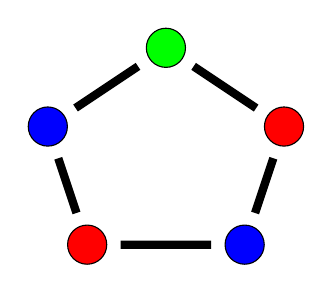
\begin{tikzpicture}[scale = 10]
\tikzstyle{VertexStyle} = []
\tikzstyle{EdgeStyle} = [line width = 3pt]
\tikzstyle{labeledStyle}=[shape = circle, minimum size = 6pt, inner sep = 1.2pt, draw]
\tikzstyle{unlabeledStyle}=[shape = circle, minimum size = 6pt, inner sep = 1.2pt, draw, fill]
\tikzstyle{cd709005-28f8-462c-809c-4d92d242e69f}=[shape = circle,minimum size = 6pt,inner sep = 5pt, outer sep = 5pt,draw,fill={rgb,255:red,255; green,0; blue,0}]
\tikzstyle{9c802e76-9af9-42f3-9bc7-eac729935b9f}=[shape = circle,minimum size = 6pt,inner sep = 5pt, outer sep = 5pt,draw,fill={rgb,255:red,0; green,0; blue,255}]
\tikzstyle{4922cc21-b00b-4fb0-85be-3c6ecc4346c7}=[shape = circle,minimum size = 6pt,inner sep = 5pt, outer sep = 5pt,draw,fill={rgb,255:red,0; green,255; blue,0}]
\Vertex[style = cd709005-28f8-462c-809c-4d92d242e69f, x = 1.150, y = 0.400, L = \tiny {}]{v0}
\Vertex[style = 9c802e76-9af9-42f3-9bc7-eac729935b9f, x = 1.100, y = 0.250, L = \tiny {}]{v1}
\Vertex[style = cd709005-28f8-462c-809c-4d92d242e69f, x = 0.900, y = 0.250, L = \tiny {}]{v2}
\Vertex[style = 9c802e76-9af9-42f3-9bc7-eac729935b9f, x = 0.850, y = 0.400, L = \tiny {}]{v3}
\Vertex[style = 4922cc21-b00b-4fb0-85be-3c6ecc4346c7, x = 1.000, y = 0.500, L = \tiny {}]{v4}
\Edge[label = \tiny {}, labelstyle={auto=right, fill=none}](v2)(v3)
\Edge[label = \tiny {}, labelstyle={auto=right, fill=none}](v1)(v0)
\Edge[label = \tiny {}, labelstyle={auto=right, fill=none}](v1)(v2)
\Edge[label = \tiny {}, labelstyle={auto=right, fill=none}](v4)(v3)
\Edge[label = \tiny {}, labelstyle={auto=right, fill=none}](v4)(v0)
\end{tikzpicture}
\caption{An odd cycle needs three crayons.}
\end{marginfigure}

\begin{theorem}\label{TwoColoring}
A graph is $2$-colorable just in case it contains no odd cycle.
\end{theorem}
\begin{proof}
A graph containing an odd cycle clearly can't be $2$-colored.  For the other implication, suppose
there is a graph that is not $2$-colorable and doesn't contain an odd cycle.  Then we may pick such a graph $G$ with $\card{G}$ as small as possible.
Surely, $|G| > 0$, so we may pick $v \in V(G)$.  If $x, y \in N(v)$, then $x$ is not adjacent to $y$ since then $xyz$ would be an odd cycle.
So we can construct a graph $H$ from $G$ by removing $v$ and identifying all of $N(v)$ to a new vertex $x_v$.  Any odd cycle
in $H$ would contain $x_v$ and hence give rise to an odd cycle in $G$ passing through $v$.  So $H$ contains no odd cycle. Since $|H| < |G|$, applying the theorem to $H$ gives a 2-coloring of $H$, say with red and blue
where $x_v$ gets colored red.  But this gives a 2-coloring of $G$ by coloring all vertices in $N(v)$ red and $v$ blue, a contradiction.
\end{proof}

Since detecting odd cycles is easy, this means $2$-coloring is easy. Things get more interesting when we move up to three colors.
\begin{theorem}
For $k \ge 3$, determining whether or not a graph has a $k$-coloring is a hard problem (supposing other problems we think are hard are, in fact, hard).
\end{theorem}

\section{Basic estimates}
Even though finding the minimum number of colors needed to color a graph is hard in general (supposing it is), we can still
look for lower and upper bounds on this value.  The \emph{chromatic number} $\chi(G)$ of a graph $G$ is the smallest $k$ for which $G$ is $k$-colorable.
The simplest thing we can do is give each vertex a different color.
\begin{theorem}\label{WorstUpperBound}
If $G$ is a graph, then $\chi(G) \le \card{G}$.
\end{theorem}
The only graphs that attain the upper bound in Theorem \ref{WorstUpperBound} are the \emph{complete} graphs; those in which
any two vertices are adjacent.
We can usually do much better by just arbitrarily coloring vertices, reusing colors when we can. 
The \emph{maximum degree} $\Delta(G)$ of a graph $G$ is the largest degree
of any vertex in $G$; that is 
\[\Delta(G) \DefinedAs \max_{v \in V(G)} d(v).\]

\begin{theorem}\label{SecondWorstUpperBound}
If $G$ is a graph, then $\chi(G) \le \Delta(G) + 1$.
\end{theorem}
\begin{proof}
Suppose there is a graph $G$ that is not $\parens{\Delta(G) + 1}$-colorable.  Then we may pick such a graph $G$ with $\card{G}$ as small as possible.
Surely, $\card{G} > 0$, so we may pick $v \in V(G)$.  Then $\card{G-v} < \card{G}$ and $\Delta(G-v) \le \Delta(G)$, so applying the theorem to $G-v$ gives a $\parens{\Delta(G-v) + 1}$-coloring
of $G-v$.  But $v$ has at most $\Delta(G)$ neighbors, so there is some color, say red, not used on $N(v)$, coloring $v$ red gives a $\parens{\Delta(G) + 1}$-coloring
of $G$, a contradiction.
\end{proof}

Both complete graphs and odd cycles attain the upper bound in Theorem \ref{SecondWorstUpperBound}.  Theorem \ref{TwoColoring} says
we can do better for graphs that don't contain odd cycles.  We can also do better for graphs that don't contain large complete subgraphs.
A set of vertices $S$ in a graph $G$ is a \emph{clique} if the vertices in $S$ are pairwise adjacent.
The \emph{clique number} of a graph $G$, written $\omega(G)$, is the number of vertices in a largest clique in $G$.

\begin{theorem}\label{OmegaLowerBound}
If $G$ is a graph, then $\chi(G) \ge \omega(G)$.
\end{theorem}

A set of vertices $S$ in a graph $G$ is \emph{independent} if the vertices in $S$ are pairwise non-adjacent.
The \emph{independence number} of a graph $G$, written $\alpha(G)$, is the number of vertices in a largest independent set in $G$.

\section{Brooks' theorem}
\begin{theorem}
If $G$ is a graph with $\Delta(G) \ge 3$ and $\omega(G) \le \Delta(G)$, then $\chi(G) \le \Delta(G)$.
\label{BrooksTheorem}
\end{theorem}
\begin{proof}
Suppose there is a graph $G$  with $\Delta(G) \ge 3$ and $\omega(G) \le \Delta(G)$ that is not $\Delta(G)$-colorable.  
Then we may pick such a graph $G$ with $\card{G}$ as small as possible.  Let $S$ be 
a maximal independent set in $G$.  Since $S$ is maximal, every vertex in $G-S$ has a neighbor in $S$, so $\Delta(G) > \Delta(G-S)$.
If red is an unused color in a $\chi(G-S)$-coloring of $G-S$, then by coloring all vertices in $S$ red we get a $\parens{\chi(G-S)+1}$-coloring of $G$.  
So, $\Delta(G) + 1 \le \chi(G) \le \chi(G-S) + 1$. We conclude $\chi(G-S) > \Delta(G - S)$ and thus $\Delta(G) = \chi(G-S) = \Delta(G-S) + 1$ by Theorem \ref{SecondWorstUpperBound}.
Since $\card{G-S} < \card{G}$, applying the theorem to $G-S$ shows that $\Delta(G-S) < 3$ or $\Delta(G -S) < \omega(G - S)$.  
So, either $\chi(G-S) = \Delta(G) = 3$ or $\omega(G-S) \ge \Delta(G)$.  In the former case, let $X$ be the vertex set of an odd cycle in $G-S$ guaranteed by Theorem \ref{TwoColoring}.  
In the latter case, let $X$ be a $\Delta(G)$-clique in $G-S$.

Since $S$ is maximal and $\omega(G) \le \Delta(G)$, there are $x_1, x_2 \in X$ and $y_1, y_2 \in S$ such that $x_1$ is adjacent to $y_1$ and $x_2$ is adjacent to $y_2$.
Construct a graph $H$ from $G-X$ by adding the edge $y_1y_2$.  Since $\card{H} < \card{G}$, applying the theorem to $H$ shows that $\omega(H) > \Delta(G)$ or $\chi(H) \le \Delta(G)$.
Suppose $\chi(H) \le \Delta(G)$.  Then there is a $\Delta(G)$-coloring of $G-X$ where $y_1$ and $y_2$ receive different colors, say red and blue respectively.
Pick the first vertex $z$ in a shortest path $P$ from $x_1$ to $x_2$ in $X$ that has a blue colored neighbor in $V(H)$. 
Each vertex in $X$ has $\Delta(G)-1$ neighbors in $X$ and hence at most one neighbor in $V(H)$.  So, $z \ne x_1$ since $x_1$ already has a red colored neighbor in $V(H)$.
Let $w$ be be the vertex preceding $z$ on $P$. Then $w$ has no blue colored neighbor.  Since $X$ is the vertex set of a cycle or a 
complete graph, there is a path $Q$ from $w$ to $z$ passing through every vertex of $X$.  Color $w$ blue and then proceed along $Q$, coloring one vertex at a time.  
Since each vertex we encounter before we get to $z$ has at most $\Delta(G) - 1$ colored neighbors, we always have an available color to use.  But, $z$ is adjacent
to both $w$ and another blue colored vertex in $V(H)$, so there is an available color for $z$ as well.  This gives a $\Delta(G)$-coloring of $G$, a contradiction.

So, $\omega(H) > \Delta(G)$.  In particular, $y_1$ and $y_2$ each have exactly one neighbor in $X$ and $\Delta(G) - 1$ neighbors in the same $\Delta(G) -1$ clique $A$ in $G - X$.
 Since $S$ is maximal and $\card{X} \ge 3$, there must be adjacent
$x_3 \in X \setminus \set{x_1,x_2}$ and $y_3 \in S \setminus \set{y_1,y_2}$.  Applying the same argument with $x_3, y_3$ in place of $x_2, y_2$ shows
that $y_1$ and $y_3$ each have exactly one neighbor in $X$ and $\Delta(G) - 1$ neighbors in the same $\Delta(G) -1$ clique $B$ in $G - X$.
Now $\card{A\cap B} = \card{A} + \card{B} - \card{A\cup B} \ge 2(\Delta(G) - 1) - d(y_1) \ge \Delta(G) - 2 > 0$.  But there can't be a vertex
in $A \cap B$ since it would be adjacent to $y_1,y_2,y_3$ as well as $\Delta(G) - 2$ vertices in $A$ and thus have degree greater than $\Delta(G)$, a contradiction. 
\end{proof}

\section{List coloring}
When attempting to $k$-color a graph $G$, it will often be convenient to first $k$-color $G[S]$ for some $S \subset V(G)$ and then try to 
$k$-color $G-S$ in a compatible manner. To make this precise, think of each vertex in $G$ starting with a list of $k$ permissible colors, say $\irange{k}$.
When we $k$-color $G[S]$, the colors used on $N(v) \cap S$ are no longer permissible for each $v \in V(G-S)$.  For $v \in V(G-S)$, let $L(v)$ be the permissible colors
for $v$ after $k$-coloring $G[S]$.  Now our problem is to pick $c_v \in L(v)$ for each $v \in V(G-S)$ such that $c_x \ne c_y$ whenever $xy \in E(G-S)$.  This is the
\emph{list coloring} problem.

The list coloring problem arose as a subproblem in our attempt to $k$-color a graph.  By taking it out of this context and viewing list coloring as a first-class problem in its own
right, we will be able to prove more general theorems while also simplifying proofs.  A \emph{list assignment} on a graph $G$ gives a set of colors $L(v)$ to each $v \in V(G)$.  
If there is $c_v \in L(v)$ for each $v \in V(G)$ such that $c_x \ne c_y$ whenever $xy \in E(G)$, then $G$ is \emph{$L$-colorable}.

\begin{theorem}\label{FirstListBound}
If $L$ is a list assignment on a graph $G$ such that $\card{L(v)} > d(v)$ for all $v \in V(G)$, then $G$ is $L$-colorable.
\end{theorem}
\begin{proof}
Color each vertex in turn using a color in its list not appearing on any of its colored neighbors.  
This succeeds since each vertex has more permissible colors than neighbors.
\end{proof}

The requirement $\card{L(v)} > d(v)$ in Theorem \ref{FirstListBound} is quite strong, in the algorithm we really only need $L(v)$ to have more colors 
than \emph{colored} neighbors rather than more colors than neighbors.  We can encode this extra information by \emph{orienting} the edges of $G$; that is, turning
each edge into an arrow pointed one way or the other.  If $G$ is an oriented graph, the \emph{out-degree} of a vertex $v \in V(G)$, written $d^+(v)$, is the number of arrows
pointing away from $v$.  An oriented graph is \emph{acyclic} if there is no sequence of arrows that ends where it starts.  An oriented graph is $L$-colorable just in case its
underlying undirected graph is $L$-colorable.

\begin{theorem}\label{SecondListBound}
If $L$ is a list assignment on an acyclic oriented graph $G$ such that $\card{L(v)} > d^+(v)$ for all $v \in V(G)$, then $G$ is $L$-colorable.
\end{theorem}
\begin{proof}
Suppose there is a list assignment $L$ on an acyclic oriented graph $G$ such that $\card{L(v)} > d^+(v)$ for all $v \in V(G)$, but $G$ is not $L$-colorable.  Then
we may pick such an $L$ and $G$ with $\card{G}$ as small as possible.  Plainly, $\card{G} \ge 2$. Since $\card{G}$ is finite and $G$ is acyclic, there must be $w \in V(G)$ with $d^+(w) = 0$.
Since $\card{L(w)} > d^+(w)$, we may choose $c \in L(w)$ and color $w$ with $c$.  Now let $L'$ be the list assignment on $G-w$ where $L'(v) = L(v) \setminus \set{c}$ if $v$
is adjacent to $w$ and $L'(v) = L(v)$ otherwise.  Since $d^+(w) = 0$, for any vertex $v$ of $G-w$ that lost $c$ from its list, we have $d_{G-w}^+(v) = d^+(v) - 1$, so 
$\card{L'(v)} > d_{G-w}^+(v)$ for all $v \in V(G-w)$.  Since $\card{G-w} < \card{G}$ and $G-w$ is also acyclic, applying the theorem shows that $G-w$ is $L'$-colorable, but then we have an $L$-coloring
of $G$, a contradiction.
\end{proof}

Theorem \ref{SecondListBound} is no longer true if we drop ``acyclic'' from the hypotheses; take a cyclically directed triangle for example.  
But there are ways to replace ``acyclic'' with weaker hypotheses and still get a true theorem.  In outline-form, the proof of Theorem \ref{SecondListBound} went like this: 
find a vertex $w$ we can color with some color $c$ such that $G-w$ is still acyclic and any vertex in $G-w$ that loses $c$ from its list also has its out-degree go down. 
This can be generalized in a couple natural ways.  First, we could color an independent set $I$ of vertices with $c$ instead of just a single vertex.  Second, we could replace ``acyclic'' with
some other property of oriented graphs, say a made-up property ``agliplic'', and require that $G-I$ remain agliplic.

It will be convenient to work with an equivalent dual version of list assignments.  
Instead of assigning a list of colors to each vertex, we assign a set of vertices to each color.  Given a set of colors $P$, a \emph{$P$-assignment} on a graph $G$ is a function
from $P$ to the subsets of $V(G)$.  For a list assignment $L$ on $G$ and $S \subseteq V(G)$, put $L(S) \DefinedAs \bigcup_{v \in S} L(v)$.
Then $L$ gives rise to the $L(V(G))$-assignment $C_L$ given by $C_L(c) \DefinedAs \setb{v}{V(G)}{c \in L(v)}$.


\begin{observation}
$G$ is $L$-colorable just in case there are independent sets $I_c \subseteq C_L(c)$ for each $c \in L(V(G))$ that together cover $V(G)$.
\end{observation}

Viewing a list assignment in this dual fashion, there is a natural candidate for a choice of $I$ to color with $c$ when trying to prove Theorem \ref{SecondListBound} for agliplic oriented graphs.
We want to find independent $I \subseteq C_L(c)$ such that every $v \in C_L(c) \setminus I$ has an out-neighbor in $I$.  Such an $I$ is a \emph{kernel} in $G\brackets{C_L(c)}$.  
So, we could try taking agliplic to mean ``$G\brackets{C_L(c)}$ has a kernel $I_c$ for all $c \in L(V(G))$''.  
That almost works, but we have no way of guaranteeing that $G-I_c$ is still agliplic.  We can fix that by requiring that $G[S]$ have a kernel for \emph{every} $S\subseteq V(G)$.  
Instead of agliplic, we call an oriented graph with this property \emph{kernel-perfect}.

\begin{theorem}\label{KernelPerfectListBound}
If $L$ is a list assignment on a kernel-perfect oriented graph $G$ such that $\card{L(v)} > d^+(v)$ for all $v \in V(G)$, then $G$ is $L$-colorable.
\end{theorem}
\begin{proof}
Suppose there is a list assignment $L$ on a kernel-perfect oriented graph $G$ such that $\card{L(v)} > d^+(v)$ for all $v \in V(G)$, but $G$ is not $L$-colorable.  Then
we may pick such an $L$ and $G$ with $\card{G}$ as small as possible.  Pick $c \in L(V(G))$ and let $I$ be a kernel in $G\brackets{C_L(c)}$.  Color all vertices in $I$ with $c$
and let $L'$ be the list assignment on $G-I$ where $L'(v) = L(v) \setminus \set{c}$ if $v \in C_L(c)$ and $L'(v) = L(v)$ otherwise.  
Since every $v \in C_L(c)$ has an out-neighbor in $I$, we have $d_{G-I}^+(v) \le d^+(v) - 1$ , so 
$\card{L'(v)} > d_{G-I}^+(v)$ for all $v \in V(G-I)$.  Since $\card{G-I} < \card{G}$ and $G-I$ is also kernel-perfect, applying the theorem shows that $G-I$ is $L'$-colorable, 
but then we have an $L$-coloring of $G$, a contradiction.
\end{proof}

Given an oriented graph $G$ that is not kernel-perfect, it is always possible to add arrows (possibly going the opposite way as a current arrow, forming a directed digon) 
to get what we'll call a \emph{superoriented graph} that is kernel-perfect.  One way is just to add back arrows for each arrow, then any maximal independent set is a kernel.
Theorem \ref{KernelPerfectListBound} holds for superoriented graphs by a nearly identical proof.  
This can be useful as it gives us a way to trade in some slack in the $\card{L(v)} > d^+(v)$ bounds for kernel-perfection by adding some extra arrows.\marginnote{\textcolor{blue}{example, picture}}

\begin{theorem}\label{KernelPerfectSuperListBound}
If $L$ is a list assignment on a kernel-perfect superoriented graph $G$ such that $\card{L(v)} > d^+(v)$ for all $v \in V(G)$, then $G$ is $L$-colorable.
\end{theorem}

\begin{lemma}\label{KostochkaYanceyKernelLemma}
If $G$ is a superoriented graph with an independent set $I$ such that all edges in $G-I$ have back arrows, then $G$ is kernel-perfect.
\end{lemma}
\begin{proof}
Suppose there is a non-kernel-perfect superoriented graph $G$ with independent set $I$ such that all edges in $G-I$ have back arrows.  Then we may pick such a $G$ with $\card{G}$
as small as possible.  Since $G$ is not kernel-perfect, there is $X \subseteq V(G)$ such that $G[X]$ has no kernel.  If $\card{X} < \card{G}$, 
then we could apply the theorem to $G[X]$ to get a kernel, so we must have $X = V(G)$.  So $I$ is not a kernel in $G$ and hence there is $v \in V(G-I)$ 
with none of its incident arrows pointing into $I$.  Remove $v$ and all its neighbors from $G$ to get a superoriented graph $H$. Since $\card{H} < \card{G}$, we may apply the
theorem to $H$ to get a kernel $S$ in $H$.  But then $S \cup \set{v}$ is a kernel in $G$ since any vertex other than $v$ in $G-H$ is either in $I$ and hence 
has an arrow to $v$ or is in $G-I$ and hence has a back arrow to $v$, a contradiction.
\end{proof}

\begin{question}
Lemma \ref{KostochkaYanceyKernelLemma} says that if we take a graph $G$ with an independent set $I$ and direct all the edges of $G-I$ both ways and the edges 
between $I$ and $V(G-I)$ arbitrarily, we get a kernel-perfect superoriented graph.  Can we classify the pairs $(G, F)$ where $G$ is a graph and $F \subseteq E(G)$ such that
every superorientation of $G$ in which all edges in $F$ are bidirected are kernel-perfect?  \marginnote{\textcolor{blue}{examples}}
\end{question}

An acylic oriented graph is plainly kernel-perfect, so Theorem \ref{KernelPerfectListBound} generalizes Theorem \ref{SecondListBound}.  
But this is not the only possible generalization of acylic that works, later\marginnote{\textcolor{blue}{what chapter?}} we will see another based on counting certain substructures of the oriented graph. 
This second generalization of acyclic does not generalize kernel-pefection and kernel-perfection does not generalize it.

\section{Historical notes}

\chapter{Flows}
Using Theorem \ref{KernelPerfectSuperListBound} and Lemma \ref{KostochkaYanceyKernelLemma}, we will prove an easily-applicable sufficient condition for a graph to be $L$-colorable.  
But first, we need a general lemma that gives graph orientations with specified constraints on their out-degrees.  This lemma can be proved directly, 
but a detour into the theory of flows will give us the lemma and many other results for free.

Let $V$ be a finite set.  A \emph{network} on $V$ is a function $\func{f}{V\times V}{\Q_{\ge 0}}$.  For a network $f$ and $X,Y \subseteq V$, put
\[\card{X,Y}_f \DefinedAs \sum_{(x,y) \in X\times Y} f(x,y).\]
If $f$ and $g$ are networks on $V$, then $f \le g$ just in case $f(u,v) \le g(u,v)$ for all $(u,v)\in V\times V$.
Let $s,t \in V$ be two distinguished vertices.  The \emph{capacity} of a network $f$, written $\card{f}$, is the minimum of $\card{X, V\setminus X}_f$ over all $X \subseteq V\setminus\set{t}$ with $s \in X$.

We call a network $f$ a \emph{flow} if $\card{\set{v},V}_f = \card{V,\set{v}}_f$ for all $v \in V \setminus \set{s,t}$.
The \emph{value} of a flow $f$ is $\size{f} \DefinedAs \card{\set{s},V}_f - \card{V,\set{s}}_f$.

\begin{lemma}\label{FlowValues}
If $f$ is a flow, then $\size{f} = \card{X, V}_f - \card{V, X}_f$ for every $X \subseteq V\setminus\set{t}$ with $s \in X$.
\end{lemma}
\begin{proof}
\begin{align*}
\card{X, V}_f - \card{V, X}_f &= \card{\set{s}, V}_f + \card{X\setminus\set{s}, V}_f - \card{V, \set{s}}_f - \card{V, X\setminus\set{s}}_f\\
&= \size{f} + \card{X\setminus\set{s}, V}_f - \card{V, X\setminus\set{s}}_f\\
&= \size{f}.
\end{align*}
\end{proof}

\begin{lemma}\label{FlowAtMostCapacity}
If $f \le g$ where $f$ is a flow on $V$ and $g$ is a network on $V$, then $\size{f} \le \card{g}$.
\end{lemma}
\begin{proof}
Pick $X \subseteq V\setminus\set{t}$ with $s \in X$ such that $\card{X, V\setminus X}_g = \card{g}$.  Then, by Lemma \ref{FlowValues}, 
\begin{align*}
\size{f} &= \card{X, V}_f - \card{V, X}_f \\
&= \card{X, V\setminus X}_f + \card{X,X}_f - \card{V\setminus X, X}_f - \card{X,X}_f \\
&= \card{X, V\setminus X}_f - \card{V\setminus X, X}_f\\
&\le \card{X, V\setminus X}_g \\
&= \card{g}.
\end{align*}
\end{proof}

\begin{theorem}\label{MaxFlowMinCut}
If $g$ is a network on $V$, then there exists a flow $f$ on $V$ with $f \le g$ such that $\size{f} = \card{g}$.
Moreover, if $g$ takes only integer values, then the flow $f$ can be chosen to as well.
\end{theorem}
\begin{proof}
Let $g$ be a network on $V$ and choose a flow $f \le g$ maximizing $\size{f}$.  By Lemma \ref{FlowAtMostCapacity}, $\size{f} \le \card{g}$.
Let $X \subseteq V$ be the set of all $v \in V$ for which there is a sequence of distinct vertices $s = x_0, x_1, x_2, \ldots, x_n = v$ such that for each $0 \le i < n$, either
$f(x_i, x_{i+1}) < g(x_i, x_{i+1})$ or $f(x_{i+1}, x_i) > 0$.  Plainly $s \in X$.

Suppose $t \in X$ and let $s = x_0, x_1, x_2, \ldots, x_n = t$ be a sequence witnessing this fact.  
Choose $\epsilon > 0$ such that for each $0 \le i < n$, either $f(x_i, x_{i+1}) \le g(x_i, x_{i+1}) - \epsilon$ or $f(x_{i+1}, x_i) \ge \epsilon$.  Modify $f$ to get $f'$
by setting $f'(x_i, x_{i+1}) = f(x_i, x_{i+1}) + \epsilon$ if $f(x_i, x_{i+1}) \le g(x_i, x_{i+1}) - \epsilon$ and $f'(x_{i+1}, x_i) = f(x_{i+1}, x_i) -\epsilon$ otherwise.
Then $f'$ is a flow with $f' \le g$ and $\size{f'} > \size{f}$, violating maximality of $\size{f}$.

So, $t \not \in X$.  Since $v \in V \setminus X$ is not in $X$, we must have $f(x, v) = g(x,v)$ and $f(v,x) = 0$ for all $x \in X$.  Hence
\begin{align*}
\size{f} &= \card{X, V}_f - \card{V, X}_f \\
&= \card{X, X}_f + \card{X, V\setminus X}_f - \card{X, X}_f - \card{V\setminus X, X}_f\\
&= \card{X, V\setminus X}_f - \card{V\setminus X, X}_f\\
&= \card{X, V\setminus X}_g\\
&\ge \card{g}.
\end{align*}
\end{proof}

\section{Hall's theorem}
As our first application of Theorem \ref{MaxFlowMinCut}, we give a sufficient condition for a graph $G$ to be $L$-colorable.  This 
condition is also necessary when $G$ is complete.
\begin{lemma}
If $L$ is a list assignment on a graph $G$ such that $\card{L(S)} \ge \card{S}$ for all $S \subseteq V(G)$, then $G$ is $L$-colorable.
\end{lemma}
\begin{proof}
Let $L$ be a list assignment on a graph $G$ such that $\card{L(S)} \ge \card{S}$ for all $S \subseteq V(G)$.  
We define a network $g$ on the set $Z \DefinedAs \set{s,t} \cup V(G) \cup L(V(G))$ by
\[g(a, b) \DefinedAs  \begin{cases} 
      1 & a = s \text{ and } b \in  V(G))\\
      1 & a = t \text{ and } b \in  L(V(G)),\\
	  1 & a \in V(G) \text{ and } b \in L(a),\\
      0 & \text{otherwise} .
   \end{cases}
\]
Let $X \subseteq Z \setminus \set{t}$ with $s \in X$.  If $P = X \cap L(V(G))$ and $Q = X \cap V(G)$, then
\begin{align*}
\card{X, Z\setminus X}_g &= \card{P, Z\setminus X}_g + \card{Q, Z\setminus X}_g + \card{\set{s}, Z\setminus X}_g\\
&\ge \card{P, Z\setminus X}_g + \card{Q} - \card{P} + \card{\set{s}, Z\setminus X}_g\\
&=\card{P} + \card{Q} - \card{P} + \card{V(G)\setminus Q}\\
&=\card{Q} + \card{V(G)\setminus Q}\\
&= \card{G}.
\end{align*}
Hence $\card{g} \ge \card{G}$.  By Theorem \ref{MaxFlowMinCut}, there is a flow $f$ on $Z$ with $f \le g$ such that $\size{f} = \card{g}$.  But then
\begin{align*}
\card{\set{s}, V(G)}_f &=  \card{\set{s}, Z}_f \\
&= \card{\set{s}, Z}_f - \card{Z, \set{s}}\\
&=\size{f}\\
&= \card{g}\\
&\ge\card{G}.
\end{align*}
Hence $f(s,v) = 1$ for all $v \in V(G)$.  Since $f$ is a flow, for each $v \in V(G)$, there is $c_v \in L(V(G))$ such that $g(v, c_v) \ge f(v, c_v) = 1$ and hence $c_v \in L(v)$.
Coloring each $v \in V(G)$ with $c_v$ gives an $L$-coloring of $G$ since if $c_v = c_w$, the fact that $f$ is a flow implies 
$\card{Z, \set{c_v}} = \card{\set{c_v}, Z} = f(c_v, t) = 1$ and hence $v = w$.
\end{proof}

\section{Orientations with prescribed degrees}
\begin{lemma}\label{InOrientations} If $G$ is a graph and $\func{g}{V(G)}{\IN}$,
then $G$ has an orientation such that $d^{-}(v)\ge g(v)$ for all $v\in V(G)$ just in case
\[
\size{X}+\size{X,V(G)\setminus X}\ge g(X),
\]
for every $X \subseteq V(G)$.
\end{lemma}

\section{Connectivity}
\section{Historical notes}

\chapter{Kernel magic}
\section{Brooks' theorem for list coloring}
\section{Triangle-free graphs}
\section{Historical notes}

\chapter{Combinatorial nullstellensatz}

Fix an arbitrary field $\mathbb{F}$. We write $f_{k_1, \ldots, k_n}$ for the coefficient of $x_1^{k_1}\cdots x_n^{k_n}$ in the polynomial $f \in \mathbb{F}[x_1, \ldots, x_n]$. 
\begin{lemma}
Suppose $f \in \mathbb{F}[x_1, \ldots, x_n]$ and $k_1, \ldots, k_n \in \IN$ with $\sum_{i \in \irange{n}} k_i = \deg(f)$.  If $f_{k_1, \ldots, k_n} \ne 0$, then for any $A_1, \ldots, A_n \subseteq \mathbb{F}$ with $\card{A_i} \ge k_i + 1$, there exists $(a_1, \ldots, a_n) \in A_1 \times \cdots \times A_n$ with $f(a_1, \ldots, a_n) \ne 0$.
\end{lemma}
\begin{proof}
Suppose the result is false and choose $f \in \mathbb{F}[x_1, \ldots, x_n]$ for which it fails 
minimizing $\deg(f)$. Then $\deg(f) \ge 2$ and we have $k_1, \ldots, k_n \in \IN$ with $\sum_{i \in \irange{n}} k_i = \deg(f)$ and 
$A_1, \ldots, A_n \subseteq \mathbb{F}$ with $\card{A_i} \ge k_i + 1$ such that $f(a_1, \ldots, a_n) = 0$ for all $(a_1, \ldots, a_n) \in A_1 \times \cdots \times A_n$.  
By symmetry, we may assume that $k_1 > 0$.  Fix $a \in A_1$ and divide $f$ by $x_1 - a$ to get $f = (x_1 - a)Q + R$ where the degree of $x_1$ in $R$ is zero.  
Then the coefficient of $x_1^{k_1-1}x_2^{k_2} \cdots x_n^{k_n}$ in $Q$ must be non-zero and $\deg(Q) < \deg(f)$.  So, by minimality of $\deg(f)$ there 
is $(a_1, \ldots, a_n) \in (A_1 \setminus \set{a}) \times \cdots \times A_n$ such that $Q(a_1,\ldots, a_n) \ne 0$.  
Since $0 = f(a_1,\ldots, a_n) = (a_1 - a)Q(a_1,\ldots, a_n) + R(a_1,\ldots, a_n)$ we must have $R(a_1,\ldots, a_n) \ne 0$.  
But $x_1$ has degree zero in $R$, so $R(a,\ldots, a_n) = R(a_1,\ldots, a_n) \ne 0$.  
Finally, this means that $f(a,\ldots, a_n) = (a-a)Q(a,\ldots, a_n) + R(a,\ldots, a_n) \ne 0$, a contradiction.
\end{proof}

\section{The graph polynomial}
Let $G$ be a loopless multigraph with vertex set $V \DefinedAs \set{x_1, \ldots, x_n}$ and edge multiset $E$.  The \emph{graph polynomial} of $G$ is
\[p_G(x_1,\ldots,x_n) \DefinedAs \prod_{\substack{\set{x_i,x_j} \in E\\i < j}} (x_i - x_j).\]
To each orientation $\vec{G}$ of $G$, there is a corresponding monomial $m_{\vec{G}}(x_1,\ldots, x_n)$ given by choosing either $x_i$ or $-x_j$ from each factor $(x_i - x_j)$ according to $\vec{G}$. Precisely, given an orientation $\vec{G}$ of $G$ with edge multiset $\vec{E}$, put
\[m_{\vec{G}}(x_1,\ldots, x_n) \DefinedAs \parens{\prod_{\substack{(x_i,x_j) \in \vec{E}\\i < j}} x_i}\parens{\prod_{\substack{(x_j,x_i) \in \vec{E}\\i < j}} -x_j}.\]
Then $p_G(x_1,\ldots,x_n) = \sum_{\vec{G}} m_{\vec{G}}(x_1,\ldots, x_n)$, where the sum is over all orientations $\vec{G}$ of $G$.  

Each $m_{\vec{G}}(x_1,\ldots, x_n)$ has coefficient either $1$ or $-1$.   
We are interested in collecting up all monomials of the form $x_1^{k_1}\cdots x_n^{k_n}$.  Let $DE_{k_1,\ldots, k_n}(G)$ be the orientations of $G$ 
where $m_{\vec{G}}(x_1,\ldots, x_n) = x_1^{k_1}\cdots x_n^{k_n}$ and $DO_{k_1,\ldots, k_n}(G)$ the orientations of $G$ where $m_{\vec{G}}(x_1,\ldots, x_n) = -x_1^{k_1}\cdots x_n^{k_n}$.  
Write $p_{k_1, \ldots, k_n}(G)$ for the coefficient of $x_1^{k_1}\cdots x_n^{k_n}$ in $p_G(x_1,\ldots,x_n)$.  Then we have
\[p_{k_1, \ldots, k_n}(G) = |DE_{k_1,\ldots, k_n}(G)| - |DO_{k_1,\ldots, k_n}(G)|.\]
This gives a combinatorial interpretation of the coefficients of $p_G$, but unfortunately it quantifies over all orientations of $G$.  
For applying the Combinatorial Nullstellensatz, it is useful to have a single orientation of $G$ as a certificate that $p_{k_1, \ldots, k_n}(G) \ne 0$.  
This can be achieved in terms of Eulerian subgraphs.  A digraph is Eulerian if the in-degree and out-degree are equal at every vertex.  
Let $EE(\vec{G})$ be the spanning Eulerian subgraphs of $\vec{G}$ with an even number of edges and let $EO(\vec{G})$ be the spanning Eulerian subgraphs of $\vec{G}$ with an odd number of edges.  

\begin{EulerianOrientationsLemma}
If $\vec{G}$ is an orientation of $G$, then we have
\[\card{|EE(\vec{G})| - |EO(\vec{G})|} = \card{|DE_{d_{\vec{G}}^+(x_1), \ldots, d_{\vec{G}}^+(x_n)}(G)|- |DO_{d_{\vec{G}}^+(x_1), \ldots, d_{\vec{G}}^+(x_n)}(G)|}.\]
\end{EulerianOrientationsLemma}
\begin{proof}
	For $D \in DE_{d_{\vec{G}}^+(x_1), \ldots, d_{\vec{G}}^+(x_n)}(G) \cup DO_{d_{\vec{G}}^+(x_1), \ldots, d_{\vec{G}}^+(x_n)}(G)$, let $\vec{G} \oplus D$ be the spanning subgraph of $\vec{G}$ with edge set 
	\[\setb{(x_i,x_j)}{E(\vec{G})}{(x_j,x_i) \in E(D)}.\]
	Then $\vec{G} \oplus D$ is Eulerian since all vertices have the same out-degree in $\vec{G}$ and $D$.  If $\vec{G}$ is even, this gives bijections between $DE_{d_{\vec{G}}^+(x_1), \ldots, d_{\vec{G}}^+(x_n)}(G)$ and $EE(\vec{G})$ as well as between $DO_{d_{\vec{G}}^+(x_1), \ldots, d_{\vec{G}}^+(x_n)}(G)$ and $EO(\vec{G})$.  When $\vec{G}$ is odd, the bijections are between $DE_{d_{\vec{G}}^+(x_1), \ldots, d_{\vec{G}}^+(x_n)}(G)$ and $EO(\vec{G})$ as well as between $DO_{d_{\vec{G}}^+(x_1), \ldots, d_{\vec{G}}^+(x_n)}(G)$ and $EE(\vec{G})$.  In either case, we have
\[\card{|EE(\vec{G})| - |EO(\vec{G})|} = \card{|DE_{d_{\vec{G}}^+(x_1), \ldots, d_{\vec{G}}^+(x_n)}(G)|- |DO_{d_{\vec{G}}^+(x_1), \ldots, d_{\vec{G}}^+(x_n)}(G)|}.\]
\end{proof} 
Therefore, if $\vec{G}$ is an orientation of $G$ with $d_{\vec{G}}^+(x_i) = k_i$ for all $i \in \irange{n}$, then
\[|p_{k_1, \ldots, k_n}(G)| = \card{|EE(\vec{G})| - |EO(\vec{G})|}.\]

\section{A coefficient formula}
\begin{lemma}
Suppose $f \in \mathbb{F}[x_1, \ldots, x_n]$ and $k_1, \ldots, k_n \in \IN$ with $\sum_{i \in \irange{n}} k_i = \deg(f)$.  For any $A_1, \ldots, A_n \subseteq \mathbb{F}$ with $\card{A_i} = k_i + 1$, we have
\[f_{k_1, \ldots, k_n} = \sum_{(a_1, \ldots, a_n) \in A_1 \times \cdots \times A_n} \frac{f(a_1, \ldots, a_n)}{N(a_1, \ldots, a_n)},\]
where
\[N(a_1, \ldots, a_n) \DefinedAs \prod_{i \in \irange{n}} \prod_{b \in A_i \setminus \set{a_i}} (a_i - b).\]
\end{lemma}
\begin{proof}
Let $f \in \mathbb{F}[x_1, \ldots, x_n]$ and $k_1, \ldots, k_n \in \IN$ with $\sum_{i \in \irange{n}} k_i = \deg(f)$. Also, let $A_1, \ldots, A_n \subseteq \mathbb{F}$ with $\card{A_i} = k_i + 1$.  For each $(a_1, \ldots, a_n) \in A_1 \times \cdots \times A_n$, let $\chi_{(a_1, \ldots, a_n)}$ be the characteristic function of the set $\set{(a_1, \ldots, a_n)}$; that is $\func{\chi_{(a_1, \ldots, a_n)}}{A_1 \times \cdots \times A_n}{\mathbb{F}}$ with $\chi_{(a_1, \ldots, a_n)}(x_1, \ldots, x_n) = 1$ when $(x_1, \ldots, x_n) = (a_1, \ldots, a_n)$ and $\chi_{(a_1, \ldots, a_n)}(x_1, \ldots, x_n) = 0$ otherwise.  Consider the function
\[F = \sum_{(a_1, \ldots, a_n) \in A_1 \times \cdots \times A_n} f(a_1, \ldots, a_n)\chi_{(a_1, \ldots, a_n)}.\]
Then $F$ agrees with $f$ on all of $A_1 \times \cdots \times A_n$ and hence $f - F$ is zero on $A_1 \times \cdots \times A_n$.  We will apply the Combinatorial Nullstellensatz to $f - F$ to conclude that $(f-F)_{k_1, \ldots, k_n} = 0$ and hence $f_{k_1, \ldots, k_n} = F_{k_1, \ldots, k_n}$ where  $F_{k_1, \ldots, k_n}$ will turn out to be our desired sum.  To apply the Combinatorial Nullstellensatz, we need to represent $F$ as a polynomial, we can do so by representing each $\chi_{(a_1, \ldots, a_n)}$ as a polynomial as follows.  For $(a_1, \ldots, a_n) \in A_1 \times \cdots \times A_n$, let 
\[N(a_1, \ldots, a_n) \DefinedAs \prod_{i \in \irange{n}} \prod_{b \in A_i \setminus \set{a_i}} (a_i - b).\]
\noindent Then it is readily verified that
\[\chi_{(a_1, \ldots, a_n)}(x_1, \ldots, x_n) = \frac{\prod_{i \in \irange{n}} \prod_{b \in A_i \setminus \set{a_i}} (x_i - b)}{N(a_1, \ldots, a_n)}.\]
\noindent Using this to define $F$ we get 
\[F(x_1, \ldots, x_n) = \sum_{(a_1, \ldots, a_n) \in A_1 \times \cdots \times A_n} f(a_1, \ldots, a_n)\frac{\prod_{i \in \irange{n}} \prod_{b \in A_i \setminus \set{a_i}} (x_i - b)}{N(a_1, \ldots, a_n)}.\]
Now  $\deg(F) = \sum_{i \in \irange{n}} (|A_i| - 1) = \sum_{i \in \irange{n}} k_i = \deg(f)$.  Since $f - F$ is zero on $A_1 \times \cdots \times A_n$, applying the Combinatorial Nullstellensatz to $f - F$ with $k_1, \ldots, k_n$ and sets $A_1, \ldots, A_n$ gives $(f-F)_{k_1, \ldots, k_n} = 0$ and hence 
\[f_{k_1, \ldots, k_n} = F_{k_1, \ldots, k_n} = \sum_{(a_1, \ldots, a_n) \in A_1 \times \cdots \times A_n} \frac{f(a_1, \ldots, a_n)}{N(a_1, \ldots, a_n)}.\]
\end{proof}

\section{Uniquely colorable graphs}
\section{Adding edges to simplify coefficient computation}
\section{AT preserving operations}
\section{Historical notes}

\chapter{Independent transversals}

\section{Randomly}
\section{A stronger bound}
\begin{theorem}\label{LopsidedTransversal}
Let $H$ be a graph and $V_1 \cup \cdots \cup V_r$ a partition of $V(H)$.  
Suppose there exists $t \geq 1$ such that for each $i \in \irange{r}$ and each $v \in V_i$ we have $d(v) \leq \min\set{t, \card{V_i}-t}$.  For any $S \subseteq V(H)$ with $\card{S} < \min\set{\card{V_1}, \ldots, \card{V_r}}$, there is an independent transversal $I$ of $V_1, \ldots, V_r$ with $I \cap S = \emptyset$.
\end{theorem}

In fact, a more general statement holds. 
First we need some notation. 
Write $\funcsurj{f}{A}{B}$ for a surjective function from $A$ to $B$.  
Let $G$ be a graph.  
For a $k$-coloring $\funcsurj{\pi}{V(G)}{\irange{k}}$ of $G$ and a subgraph $H$ of $G$ we say 
that $I \DefinedAs \set{x_1, \ldots, x_k} \subseteq V(H)$ is an $H$-independent transversal of $\pi$ if $I$ is an independent 
set in $H$ and $\pi(x_i) = i$ for all $i \in \irange{k}$.

\begin{lemma}\label{BaseTransversalLemma}
Let $G$ be a graph and $\funcsurj{\pi}{V(G)}{\irange{k}}$ a proper $k$-coloring of
$G$.  Suppose that $\pi$ has no $G$-independent transversal, but for every $e
\in E(G)$, $\pi$ has a $(G-e)$-independent transversal. Then for every $xy \in
E(G)$ there is $J \subseteq \irange{k}$ with $\pi(x), \pi(y) \in J$ and an 
induced matching $M$ of $G\brackets{\pi^{-1}(J)}$ with $xy \in M$ such that:
\begin{enumerate}
  \item $\bigcup M$ totally dominates $G\brackets{\pi^{-1}(J)}$,
  \item the multigraph with vertex set $J$ and an edge between $a, b \in J$ for
  each $uv \in M$ with $\pi(u) = a$ and $\pi(v) = b$ is a (simple) tree.  In
  particular $\card{M} = \card{J} - 1$.
\end{enumerate}
\end{lemma}
\begin{proof}
Suppose the lemma is false and choose a counterexample $G$ with
$\funcsurj{\pi}{V(G)}{\irange{k}}$ so as to minimize $k$.  Let $xy \in E(G)$.
By assumption $\pi$ has a $(G-xy)$-independent transversal $T$.  Note that we
must have $x,y \in T$ lest $T$ be a $G$-independent transversal of $\pi$.

By symmetry we may assume that $\pi(x) = k-1$ and $\pi(y) = k$. Put $X
\DefinedAs \pi^{-1}(k-1)$, $Y \DefinedAs \pi^{-1}(k)$ and $H \DefinedAs G -
N(\set{x, y}) - E(X,Y)$. Define $\func{\zeta}{V(H)}{\irange{k-1}}$ by $\zeta(v)
\DefinedAs \min\set{\pi(v), k-1}$. Note that since $x,y \in T$, we have
$\card{\zeta^{-1}(i)} \geq 1$ for each $i \in \irange{k-2}$.  Put $Z \DefinedAs
\zeta^{-1}(k-1)$. Then $Z \neq \emptyset$ for otherwise $M \DefinedAs \set{xy}$
totally dominates $G[X \cup Y]$ giving a contradiction.

Suppose $\zeta$ has an $H$-independent transversal $S$.  Then we have $z \in S
\cap Z$ and by symmetry we may assume $z \in X$.  But then $S \cup \set{y}$ is
a $G$-independent transversal of $\pi$, a contradiction.

Let $H' \subseteq H$ be a minimal spanning subgraph such that $\zeta$ has no
$H'$-independent transversal.  Now $d(z) \geq 1$ for each $z \in Z$ for
otherwise $T - \set{x,y} \cup \set{z}$ would be an $H'$-independent transversal
of $\zeta$.  Pick $zw \in E(H')$.  By minimality of $k$, we have $J \subseteq
\irange{k-1}$ with $\zeta(z), \zeta(w) \in J$ and an induced matching $M$ of
$H'\brackets{\zeta^{-1}(J)}$ with $zw \in M$ such that
\begin{enumerate}
  \item $\bigcup M$ totally dominates $H'\brackets{\zeta^{-1}(J)}$,
  \item the multigraph with vertex set $J$ and an edge between $a, b \in J$ for
  each $uv \in M$ with $\zeta(u) = a$ and $\zeta(v) = b$ is a (simple) tree.
\end{enumerate}

Put $M' \DefinedAs M \cup \set{xy}$ and $J' \DefinedAs J \cup \set{k}$.
Since $H'$ is a spanning subgraph of $H$, $\bigcup M$ totally dominates
$H\brackets{\zeta^{-1}(J)}$ and hence $\bigcup M'$ totally dominates
$G\brackets{\pi^{-1}(J')}$.  Moreover, the multigraph in (2) for $M'$ and $J'$
is formed by splitting the vertex $k-1 \in J$ into two vertices and adding an edge
between them and hence it is still a tree.  This final contradiction proves the
lemma.
\end{proof}

\begin{proof}[Proof of Theorem \ref{LopsidedTransversal}]
Suppose the lemma fails for such an $S \subseteq V(H)$.  Put $H' \DefinedAs H - S$ and let $V_1', \ldots, V_r'$ be the induced partition of $H'$. Then there is no independent transversal of $V_1', \ldots, V_r'$ and $\card{V_i'} \geq 1$ for each $i \in \irange{r}$. Create a graph $Q$ by removing edges from $H'$ until it is edge minimal without an independent transversal. Pick $yz \in E(Q)$ and apply Lemma 
\ref{BaseTransversalLemma} on $yz$ with the induced partition to get the guaranteed 
$J \subseteq \irange{r}$ and the tree $T$ with vertex set $J$ and an edge between $a, b \in
J$ for each $uv \in M$ with $u \in V_a'$ and $v \in V_b'$.  By our condition, for each $uv \in E(V_i, V_j)$, we have $\card{N_H(u) \cup N_H(v)} \leq \min\set{\card{V_i}, \card{V_j}}$.

Choose a root $c$ of $T$. Traversing $T$ in leaf-first order and for each leaf $a$ with parent $b$ picking $|V_a|$ from $\min\set{|V_a|, |V_b|}$ we get that the vertices in $M$ together dominate at most $\sum_{i \in J \setminus \set{c}} \card{V_i}$ vertices in $H$.  Since $\card{S} < \card{V_c}$, $M$ cannot totally dominate $\bigcup_{i \in J} V_i'$, a contradiction.
\end{proof}

Note that the condition on $S$ can be weakened slightly.  Suppose we have ordered the $V_i$ so that $\card{V_1} \leq \card{V_2} \leq \cdots \leq \card{V_r}$.  Then for any $S \subseteq V(H)$ with $\card{S} < \card{V_2}$ such that $V_1 \not \subseteq S$, there is an independent transversal $I$ of $V_1, \ldots, V_r$ with $I \cap S = \emptyset$.  The proof is the same except when we choose our root $c$, choose it so as to maximize $\card{V_c}$.  
Since $\card{J} \geq 2$, we get $\card{V_c} \geq \card{V_2} > \card{S}$ at the end.
\section{Lists with low degree color graphs}

\section{Hitting all maximum cliques}
Let $G$ be a graph. For a collection of cliques $\Q$ in $G$, let $X_\Q$ be the intersection graph of $\Q$; that is, the 
vertex set of $X_\Q$ is $\Q$ and there is an edge between $Q_1, Q_2 \in \Q$ iff $Q_1 \ne Q_2$ and $Q_1$ and $Q_2$ intersect.
When $\Q$ is a collection of maximum cliques, we get a lot of information about $X_\Q$.  
\begin{lemma}\label{HajnalLemma}
If $G$ is a graph and $\Q$ is a collection of maximum cliques in $G$, then 
\[\card{\bigcup \Q} + \card{\bigcap \Q} \geq 2\omega(G).\]
\end{lemma}

\begin{lemma}\label{KostochkaCliqueGraph}
If $\Q$ is a collection of maximum cliques in a graph $G$ with $\omega(G) > \frac23 (\Delta(G) + 1)$ such that $X_\Q$ is connected, then $\cap \Q \neq \emptyset$. 
\end{lemma}
\begin{proof}
Suppose not and choose a counterexample $\Q \DefinedAs \set{Q_1, \ldots, Q_r}$
minimizing $r$. Plainly, $r \geq 3$. Let $A$ be a noncutvertex in $X_{\Q}$ and
$B$ a neighbor of $A$. Put $\fancy{Z} \DefinedAs \Q - \set{A}$. Then
$X_{\fancy{Z}}$ is connected and hence by minimality of $r$, $\cap \fancy{Z}
\neq \emptyset$. In particular, $\card{\cup \fancy{Z}} \leq \Delta(G) + 1$.
By assumption, $\cap\Q=\emptyset$, so $\card{\cap \Q} + \card{\cup \Q} \leq 0 +
(\card{\cup \fancy{Z}} + \card{A - B}) \leq
(\Delta(G) + 1) + (\Delta(G)+1 - \omega(G)) < 2\omega(G)$. This contradicts
Lemma \ref{HajnalLemma}.
\end{proof}

\begin{lemma}\label{TwoThirdsEqualityStructure}
If $\Q$ is a collection of maximum cliques in a graph $G$ with $\omega(G) \ge \frac23 (\Delta(G) + 1)$ such that $X_\Q$ is connected, then either 
\begin{itemize}
\item $\cap \Q \ne \emptyset$; or
\item $\Delta(X_\Q) \le 2$ and if $B, C \in \Q$ are different neighbors of $A \in \Q$, then $B \cap C = \emptyset$ and $\card{A \cap B} = \card{A \cap C} = \frac12 \omega(G)$.
\end{itemize}
\end{lemma}

\section{Strong coloring}
\section{When every vertex is in a big clique}
\section{Historical notes}

\chapter{Kempe chains and vertex shuffling}
\section{Historical notes}

\chapter{Vertex transitive graphs}
Let $G$ be a vertex-transitive graph and let $\Q$ be the collection of all
maximum cliques in $G$.  It is not hard to see that $X_\Q$ is vertex-transitive
as well; in fact, we have the following.

\begin{observation}\label{transitiveClustering}
Let $G$ be a vertex-transitive graph and let $\Q$ be the collection of all
maximum cliques in $G$.  For each component $C$ of $X_\Q$, put $G_C \DefinedAs
G\brackets{\bigcup V(C)}$.  Then $G_C$ is vertex-transitive for each component
$C$ of $X_\Q$ and $G_{C_1} \cong G_{C_2}$ for components $C_1$ and $C_2$ of
$X_\Q$.
\end{observation}

\begin{lemma}\label{TransitiveClusteringBigCliques}
Let $G$ be a connected vertex-transitive graph and let $\Q$ be the collection
of all maximum cliques in $G$.  If $\omega(G) \ge \frac23 \parens{\Delta(G) +
1}$, then either
\begin{itemize}
\item $X_\Q$ is edgeless; or
\item $X_\Q$ is a cycle and $G$ is the graph obtained from $X_\Q$ by blowing up each vertex to a $K_{\frac12 \omega(G)}$.
\end{itemize}
\end{lemma}
\begin{proof}
If $\omega(G) > \frac23 \parens{\Delta(G) + 1}$, then $X_\Q$ is edgeless as shown above.  Hence we may assume $\omega(G) = \frac23 \parens{\Delta(G) + 1}$.  
Let $Z$ be a component of $X_\Q$ and put $\Z \DefinedAs V(Z)$.
By Lemma \ref{TwoThirdsEqualityStructure}, $\Delta(X_\Z) \le 2$ and if $B, C \in \Z$ are 
different neighbors of $A \in \Z$, then $B \cap C = \emptyset$ and $\card{A \cap B} = \card{A \cap C} = \frac12 \omega(G)$.  
By Observation \ref{transitiveClustering}, $X_\Z$ must be a cycle.  But then every vertex in $G_Z$ has 
$\frac12 \omega(G) + \frac12 \omega(G) + \frac12 \omega(G) - 1 = \Delta(G)$ neighbors in $G_Z$ and thus $G = G_Z$.  
Hence $X_\Q = X_\Z$ is a cycle and $G$ is the graph obtained from $X_\Q$ by blowing up each vertex to a $K_{\frac12 \omega(G)}$.
\end{proof}

\section{Historical notes}


\chapter{Coloring edges}
It is also useful to consider coloring the edges of a graph so that incident edges receive different colors.  This
appears to be at odds with our previous claim that this book was only about coloring vertices of graph; fortunately, edge coloring
is just a special case of vertex coloring.  If $G$ is a graph, the \emph{line graph} of $G$, written
$L(G)$ is the graph with vertex set $E(G)$ where two edges of $G$ are adjacent in $L(G)$ if they are incident in $G$.  Coloring
the edges of $G$ is equivalent to coloring the vertices of $L(G)$.

For graphs with maximum degree zero (that is, no edges at all), we can get by with zero colors.  
With just one color we can edge color any graph with maximum degree at most one.  We will definitely always need at least $\Delta(G)$ colors
to edge color a graph $G$.  Could we be so fortunate that the pattern continues
and we can edge color any graph $G$ with only $\Delta(G)$-colors? Not quite, but we can do so for bipartite ($2$-colorable) graphs.
A graph is $k$-edge-colorable if we can color its edges with (at most) $k$ colors such that incident edges receive different colors.
A color $c$ us $\emph{used}$\aaside{used}{} at a vertex $v$ of $G$ if an edge incident to $v$ in $G$ is colored with $c$. Otherwise, $c$ is \emph{available}\aaside{available}{} at $v$.
A \emph{path}\aaside{path}{+0.15in} in $G$ is a sequence of pairwise distinct vertices $x_1x_2\cdots x_k$ such that $x_i$ is adjacent to $x_{i+1}$ for $i \in \irange{k-1}$.

\begin{theorem}\label{DeltaEdgeColoring}
If $G$ is a bipartite graph, then $G$ is $\Delta(G)$-edge-colorable.
\end{theorem}
\begin{proof}
Suppose there is a graph $G$ that is not $\Delta(G)$-edge-colorable.  Then we may pick such a graph $G$ with $\size{G}$ as small as possible.
Now $\size{G} > 0$, since we can surely edge color a graph with zero edges using zero colors.  Let $xy$ be an edge in $G$.  Since $\size{G-xy} < \size{G}$,
applying the theorem to $G-xy$ gives an edge coloring of $G-xy$ using at most $\Delta(G)$ colors.  Now each of $x$ and $y$ are incident to at most $\Delta(G) - 1$ edges
in $G-xy$ and $G$ has no $\Delta(G)$-edge-coloring, so there is a color red available at $x$ and a different color blue available at $y$.  There is a unique maximal 
path $P$ starting at $x$ with edges alternately colored blue and red. If $P$ does not end at $y$, then we get a $\Delta(G)$-edge-coloring of $G$ by swapping the colors red and blue 
along $P$ and coloring $xy$ blue, a contradiction.  Since $P$ ends at $y$ and alternates between red and blue, it has even length.  But then $P + xy$ is an odd cycle in $G$, violating
Theorem \ref{TwoColoring}.
\end{proof}

It may come as a surpise that even though we might need more than $\Delta(G)$ colors to edge color a graph $G$, we will only ever need at most one extra color.
For bipartite graphs we were able to repair an almost correct coloring by swapping colors along a path because we had control over where this path ended.  In the
general case we don't have the same control over a path between two vertices, but we can exert some measure of control over paths leaving and entering a larger structure. 
The larger structure we use here is the whole neighborhood of a vertex.

This is a good time to introduce a lemma that will be useful throughout the book.  
A \emph{transversal} in a collection of sets $\set{A_i}_{i \in \irange{k}}$ is a set $X \subseteq \bigcup_{i \in \irange{k}} A_i$ with $\card{X} = k$ such that $\card{X \cap A_i} = 1$
for all $i \in \irange{k}$.
\begin{lemma}
$\set{A_i}_{i \in \irange{k}}$ has a transversal just in case $\card{\bigcup_{i \in I} A_i} \ge \card{I}$ for all $I \subseteq \irange{k}$.
\end{lemma}
\begin{proof}
\end{proof}

\begin{corollary}\label{TransversalCorollary}
If $\card{\bigcup_{i \in \irange{k}} A_i} \ge k$, then there is nonempty $I \subseteq \irange{k}$ such that $\set{A_i}_{i \in I}$ has a transversal $X$ where $X \cap A_i = \emptyset$
for all $i \in \irange{k} \setminus I$.
\end{corollary}
\begin{proof}
\end{proof}

\begin{theorem}
If $G$ is a graph, then $G$ is $\parens{\Delta(G) + 1}$-edge-colorable.
\end{theorem}
\begin{proof}
Suppose there is a graph $G$ that is not $(\Delta(G) + 1)$-edge-colorable.  Then we may pick such a graph $G$ with $\card{G}$ as small as possible.
Now $\card{G} > 0$, since we can surely edge color a graph with zero vertices using at most one color. Let $x$ be a vertex in $G$.   Call $S\subseteq N(x)$ \emph{acceptable} for 
an edge coloring $\pi$ of $G-x$ if $\set{\bar{\pi}(v)}_{v \in S}$ has a transversal $T_S$ such that $\card{\bar{\pi}(v) \setminus T_S} \ge 2$ for all $v \in N(x)\setminus S$.

Since $\card{G-x} < \card{G}$, applying the theorem to $G-x$ gives an edge coloring $\zeta$ of $G-x$ using at most $\Delta(G) + 1$ colors. 
Note that the empty set is acceptable for $\zeta$.  So, we may choose an edge coloring $\pi$ of $G-x$ using at most $\Delta(G) + 1$ colors and $S\subseteq N(x)$ 
that is acceptable for $\pi$ so as to maximize $\card{S}$ and subject to that to maximize $\card{C_S}$, where
\[C_S \DefinedAs \bigcup_{v \in N(x) \setminus S} \bar{\pi}(v) \setminus T_S.\]
Now $S \neq N(x)$ for otherwise we can extend $\pi$ to all of $G$ using $T_S$.  Suppose $\card{C_S}\ge \card{N(x) \setminus S}$.
Then, by Corollary \ref{TransversalCorollary}, there is nonempty $A \subseteq N(x) \setminus S$ such that $\set{\bar{\pi}(v)\setminus T_S}_{v \in A}$ has
a transversal $X$ where $X \cap \bar{\pi}(v) = \emptyset$ for all $v \in N(x) \setminus \parens{S \cup A}$.  But then $S\cup A$ is acceptable for $\pi$, contradicting
maximality of $\card{S}$.  

So, $\card{C_S}< \card{N(x) \setminus S}$ and hence $\card{C_S \cup T_S} < \card{N(x)} \le \Delta(G)$.  
Pick $\tau \in \irange{\Delta(G)} \setminus \parens{C_S \cup T_S}$.  Since $S$ is acceptable for $\pi$, $\card{\bar{\pi}(v) \setminus T_S} \ge 2$ for all $v \in N(x)\setminus S$.
Hence there are $v_1, v_2, v_3 \in N(x)\setminus S$ and $\gamma \in C_S$ such that $\gamma \in \bar{\pi}(v_i) \setminus T_S$ for all $i \in \irange{3}$.
There is a unique maximal path $P$ starting at $v_1$ with edges alternately colored $\tau$ and $\gamma$.  
Let $\zeta$ be the edge coloring made from $\pi$ by swapping $\tau$ and $\gamma$ on $P$.  Then $\zeta$ violates the maximality of $\card{C_S}$ since $S$ is acceptable for $\zeta$ and
\[\bigcup_{v \in N(x) \setminus S} \bar{\zeta}(v) \setminus T_S = \set{\tau} \cup C_S.\]

\end{proof}

\section*{hardness}
We now know that every graph $G$ can be edge colored with either $\Delta(G)$ or $\Delta(G) + 1$ colors.  So, edge coloring is basically trivial, right?
Furtunately, no it isn't, the collection of graphs requiring $\Delta(G) + 1$ colors is very rich.  Another way to say this, is that it is a hard problem
to decide whether or not edge coloring a given graph $G$ requires $\Delta(G) + 1$ colors.  

\begin{theorem}
Deciding whether or not edge coloring a given graph $G$ requires $\Delta(G) + 1$ colors is hard supposing other things we think are hard are actually hard.
\end{theorem}

\section*{fans as a greedy strategy}
\section*{acceptable paths}
\section*{acceptable trees}
\section*{edge list coloring}
\section{Historical notes}
\backmatter
\appendix
\setboolean{@mainmatter}{true}
\chapter{Basic probability}

\printindex
\end{document}